%----------------------------------------------------------------------------
%----------------------------------------------------------------------------
%%%%%%%%%%%%%%%%%%%%%%%%%%%%%%% -*- Mode: Latex -*- %%%%%%%%%%%%%%%%%%%%%%%%%%%%
%% >>slacT486/intro.tex<<
%% Author          : R. Jeffrey Kowalski
%% Created On      : Tue Apr 10 19:50:51 HST 2007
%% Last Modified On: Thu Aug  2 10:54:56 HST 2007
%%%%%%%%%%%%%%%%%%%%%%%%%%%%%%%%%%%%%%%%%%%%%%%%%%%%%%%%%%%%%%%%%%%%%%%%%%%%%%%
From June 19-24, 2006, the experiment, SLAC T486, was performed in the End Station A facility at the Stanford Linear Accelerator Center to measure the Askaryan effect in ice.  28.5 GeV electrons were accelerated with typically 10$^9$ particles in 10 picosecond bunches and delivered into a 7.5 metric tonne target of carving-grade ice to produce electromagnetic showers.  In a dense media like ice, coherent microwave Cherenkov radiation emerges from the particle shower and propagates to the surface of the target where radio antennas can detect the radiation.  This chapter outlines the T486 experiment and the analysis of the Askaryan effect in ice.
%----------------------------------------------------------------------------
%----------------------------------------------------------------------------
\section{General description}
Armed with the information from the previous chapters, we outline methods employed to condition the dye laser system for coherent control spectroscopy. This section introduces the systems used to condition a single dye laser, then outlines the method of mixing and delaying the pulses, and finally gives a brief description of the interaction region and the data acquisition chain.
%----------------------------------------------------------------------------
\subsection{Single dye laser conditioning}
%----------------------------------------------------------------------------
%----------------------------------------------------------------------------
It has become clear that the main issue one must deal with to prepare a commercial dye laser for use in a multi-color coherent control experiment is the multi-mode nature of these sources. The processes under investigation demand transform limited pulses \cite{Corless:1997a} and well controlled intensity profiles. The raw output of each of the three dye lasers is unusable since it is not transform limited, has non--Gaussian anti-symmetric transverse intensity profiles ($M^2$ not close to unity), and cannot be arbitrarily delayed with respect to the pump laser. To condition each beam for use in the experiment, we temporally condition the pulse into a Gaussian shape, run the pulse through a variable delay line, spatially filter the beam to eliminate the non-TEM00 transverse modes ($M^2 \sim 1$), then spectrally filter the pulse to its transform limit (see figure \ref{block_dye}).
%----------------------------------------------------------------------------
% block_dye.tex.tex
% by Troy Hix, May 2005
%----------------------------------------------------------------------------
\begin{figure}
\center
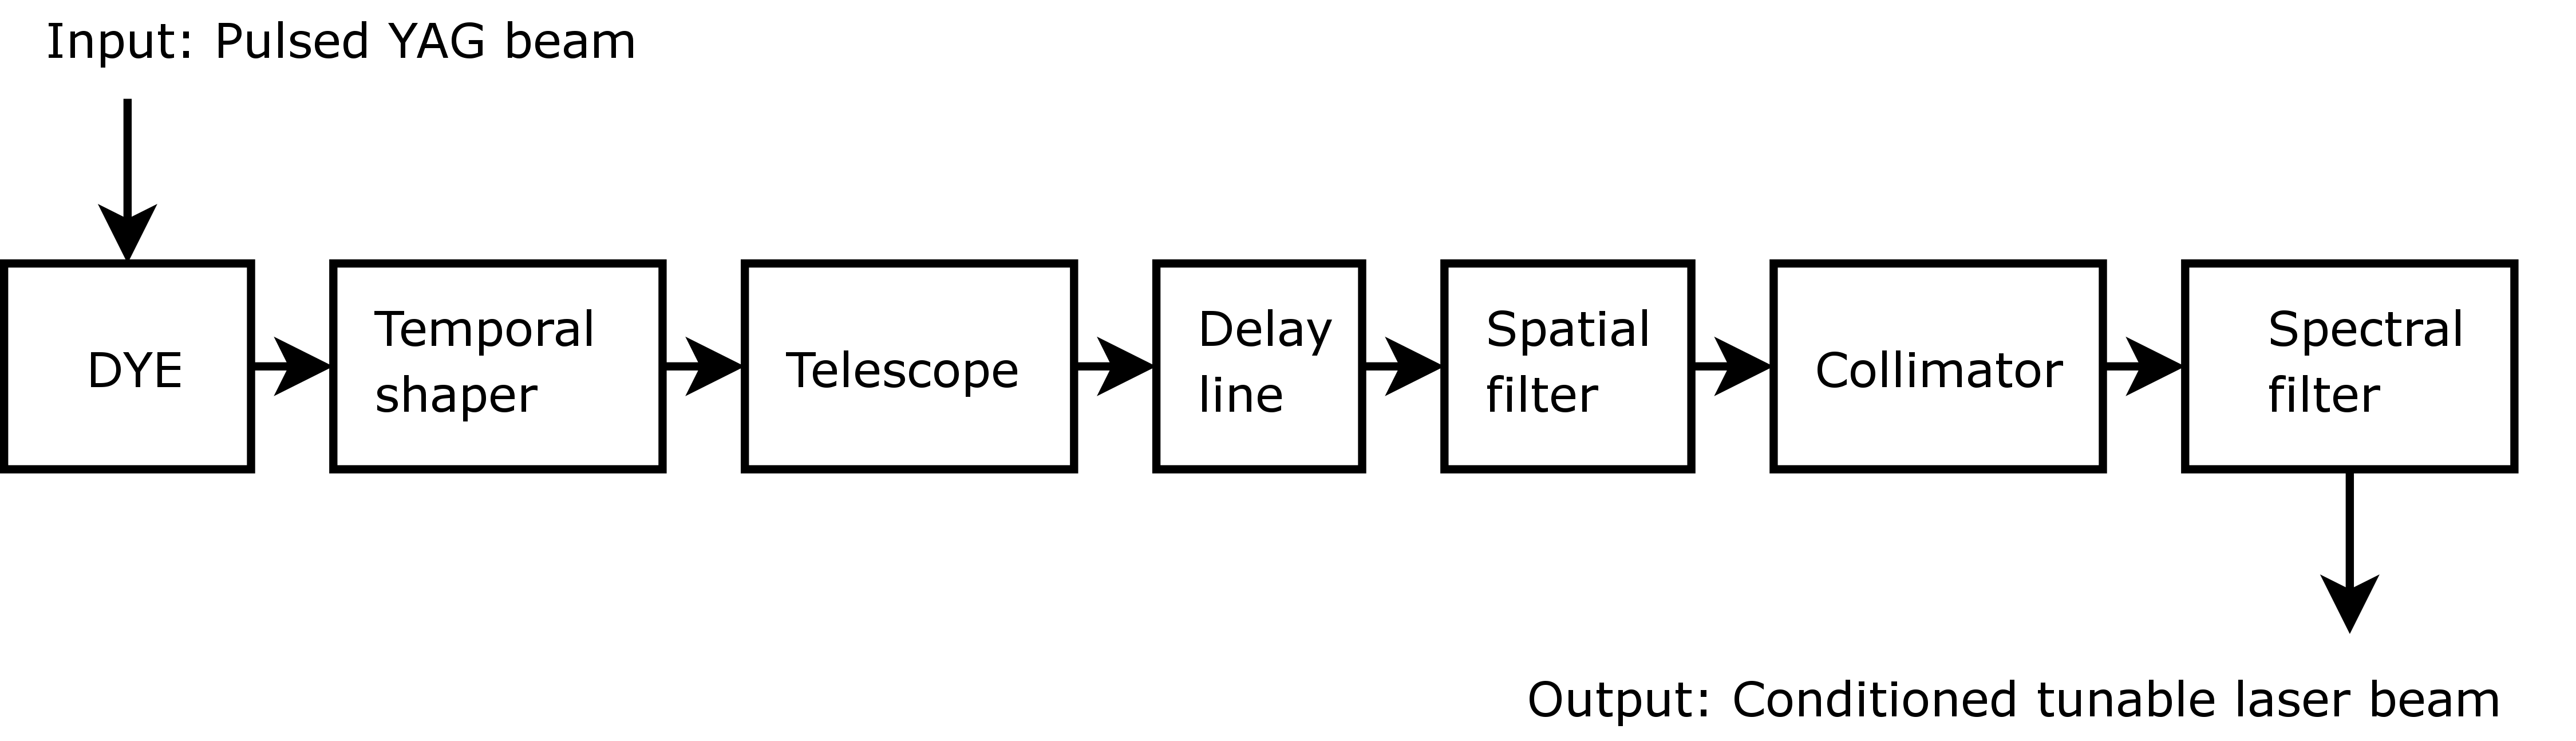
\includegraphics[width=6.00in]
{block_dye/block_dye.png}\\
\caption{Single dye laser conditioning block diagram}
\label{block_dye}
\end{figure} 
%----------------------------------------------------------------------------
%----------------------------------------------------------------------------
%----------------------------------------------------------------------------



%----------------------------------------------------------------------------

The temporal shaper is a Pockels cell (the Pockels cell will also be used to set the amplitude of each pulse). It has been shown in the lab that the Pockels cell can create dye laser pulses with widths from 0.8 ns to 4.4 ns. The lower limit is a characteristic of the Pockels cell and its associated electronics; the upper limit is roughly the longest pulse we are able to generate when we eliminate the ragged leading and trailing edges of the raw laser output. For transform limited shapes (Gaussians), the temporal FWHM of the intensity is related to the spectral FWHM of the power spectrum by
%----------------------------------------------------------------------------
\begin{equation}
\boxed{
\sigma_\nu
=
\frac
{\ln(16)}
{2\pi\sigma_t},
\label{FWHM power}
}
\end{equation}
%----------------------------------------------------------------------------
where $\sigma_\nu$ is the spectral FWHM and $\sigma_t$ is the temporal FWHM.

Thus, if $\sigma_t$ is 0.8 ns then $\sigma_\nu$ is 552 MHz, and if $\sigma_t$ is 4.4 ns then $\sigma_\nu$ is 100 MHz. These are the target spectral filter widths for long and short pulse experiments. The spectral filters are etalons with a FSR big enough to prevent aliasing and a mode width of 100 MHz to 552 MHz depending on the type of experiment.

The delay line extends the path length of the beam in such a manner to allow arbitrary delay between the dye laser pulse and YAG pump. A telescope is used upstream from the delay line to minimize the effect of the variable path length between the dye laser output and the spatial filter. The spatial filter is placed downstream from the delay line and shall consist of a focusing lens and a pinhole. The central maximum from the pinhole (Airy function) is mode matched into the etalon (beam is collimated if a planar configuration is used - or focused if confocal). Then the beam is finally collimated (if necessary) and sent to the molecular interaction region.
%----------------------------------------------------------------------------
%----------------------------------------------------------------------------
%----------------------------------------------------------------------------
%----------------------------------------------------------------------------
%----------------------------------------------------------------------------
%----------------------------------------------------------------------------

%----------------------------------------------------------------------------
\subsection{Controlled three pulse sequence}
%----------------------------------------------------------------------------
%----------------------------------------------------------------------------
The experiment requires three properly conditioned pulses, all incident upon the same spatial region, sequenced in a specific temporal order. A single Nd:YAG pulsed dye laser is used to simultaneously pump three dye lasers; thus the relative delay between each dye laser is fixed. We will obtain arbitrary control of the pulse sequence by delaying two pulses with respect to the third. By manipulating the beam line design, we can force all three pulses to be temporally coincident while the delay lines are in their middle positions. In this way each of the two delayed pulses can be retarded or advanced by 4 ns with respect to the un-delayed pulse. We can even swap dye cells between dye lasers for complete control of the color order in the pulse sequence.

Once the pulses are properly delayed and ordered, they are aligned in a ``beam mixer'' so that their optical axes are collinear. The final output of the laser system is a three color transform limited pulse sequence with user specified color triple, amplitude triple, and relative delay of the pulses within the sequence. We use a 50/50 beam splitter as the beam mixer. Since we do not yet know the optimal color sequence, in the initial stages of this experiment, we will use broadband 50/50 beam splitters as we explore different color sets. Once the optimal color sequence is set, then more efficient optics could be specified if required. See figure \ref{block_three_dye}.
%----------------------------------------------------------------------------
% block_three_dye.tex
% by Troy Hix, May 2005
%----------------------------------------------------------------------------
\begin{figure}
\center
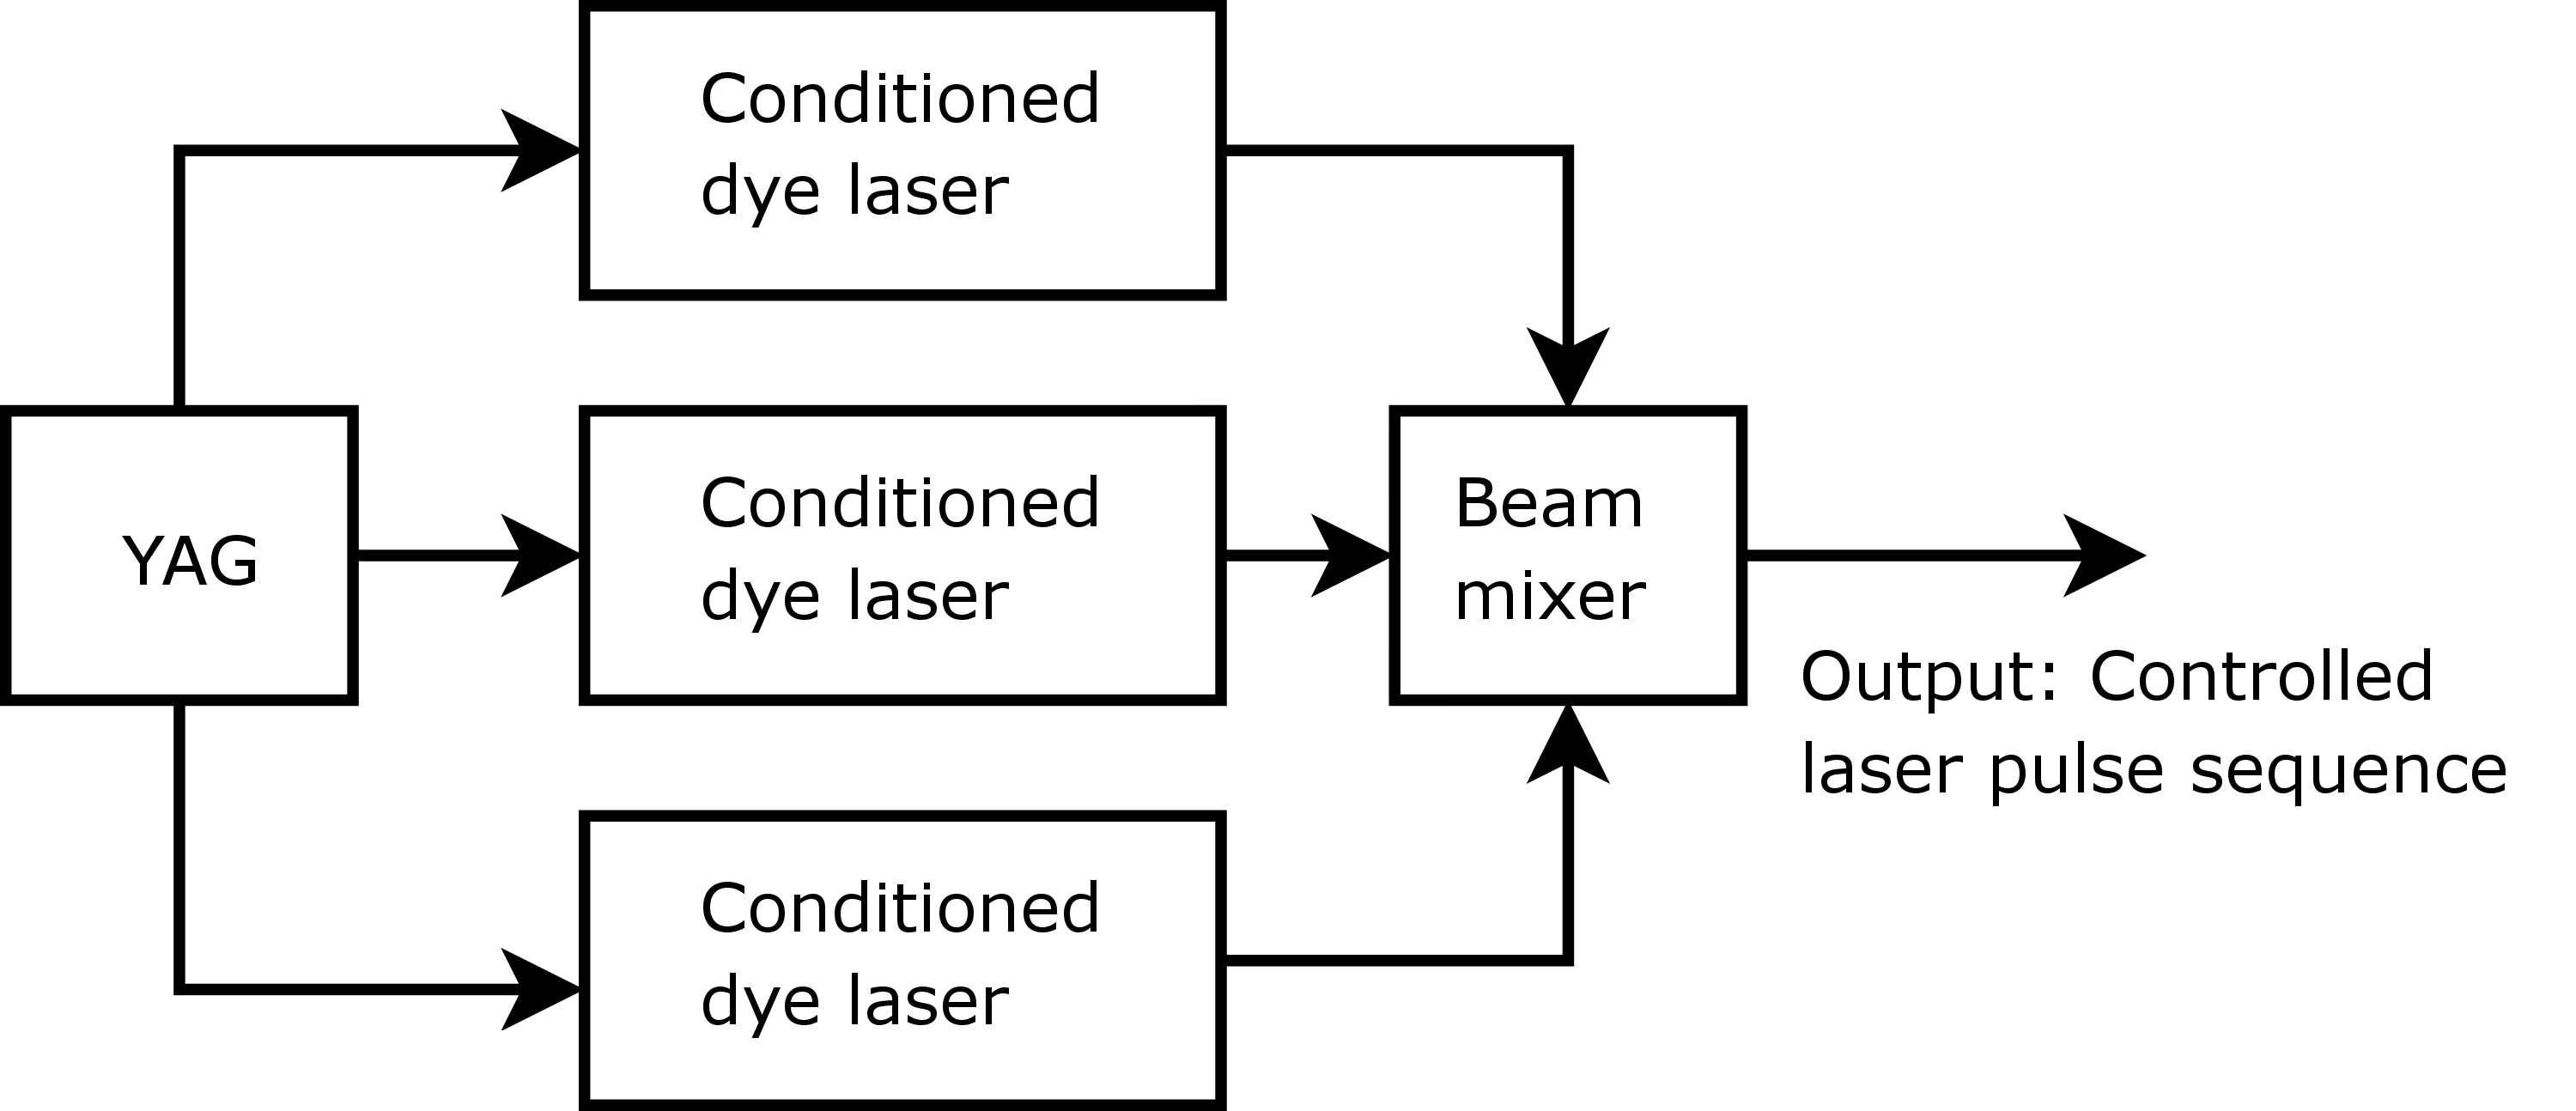
\includegraphics[width=4.00in]
{block_three_dye/block_three_dye.png}\\
\caption{Three conditioned and synchronized dye lasers block diagram}
\label{block_three_dye}
\end{figure} 
%----------------------------------------------------------------------------
%----------------------------------------------------------------------------
%----------------------------------------------------------------------------



%----------------------------------------------------------------------------
%----------------------------------------------------------------------------
%----------------------------------------------------------------------------
%----------------------------------------------------------------------------
%----------------------------------------------------------------------------

%----------------------------------------------------------------------------
\subsection{Interaction and data acquisition}
%----------------------------------------------------------------------------
%----------------------------------------------------------------------------
The collimated output of the three dye laser system is incident on a controlled sample of thermal molecular iodine. A circular aperture is placed immediately upstream from the sample to approximate a top hat spatial field in the interaction region. Initially, the sample is pure molecular iodine vapor at various concentrations - i.e., low buffer gas pressure. Once the various coherent processes of interest are verified (proof of concept), a buffer gas is introduced at various concentrations to measure the noise suppression limit of each of the coherent processes (efficiency).

The fluorescence signal from the interaction region is imaged onto the input slit of the monochromator by a lens system. The output of the monochromator may be read by either a CCD array (good for initial exploring and verification) or a PMT (temporally resolved and gated). The CCD image is directly downloaded into a PC for processing. The PMT signal is gated, amplified, and averaged (if necessary) in a gated boxcar averager system; the output of the boxcar system may then be read by either a chart recorder or a ADC equipped PC for processing. See figure \ref{block_fluorescence}.
%----------------------------------------------------------------------------
% block_fluorescence.tex
% by Troy Hix, May 2005
%----------------------------------------------------------------------------
\begin{figure}
\center
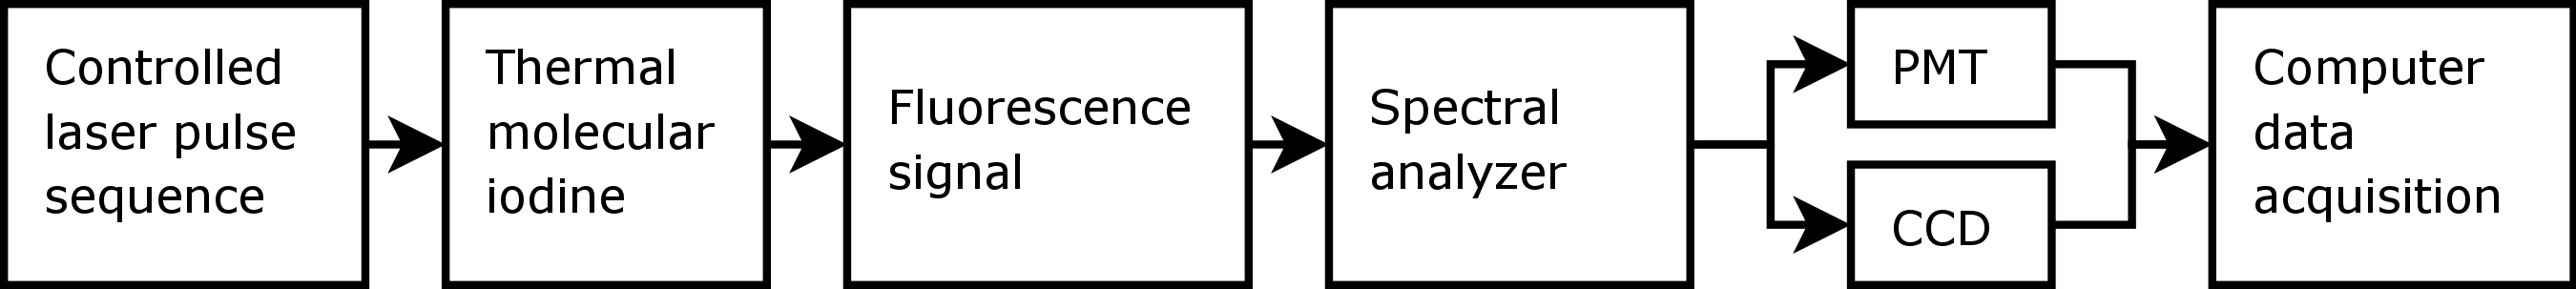
\includegraphics[width=6.00in]
{block_fluorescence/block_fluorescence.png}\\
\caption{Interaction and data acquisition block diagram}
\label{block_fluorescence}
\end{figure} 
%----------------------------------------------------------------------------
%----------------------------------------------------------------------------
%----------------------------------------------------------------------------



%----------------------------------------------------------------------------
%----------------------------------------------------------------------------
%----------------------------------------------------------------------------
%----------------------------------------------------------------------------

%----------------------------------------------------------------------------
%----------------------------------------------------------------------------
\section{Layout}
The entire system will span three optical tables: the laser beams start on the ``dye laser'' table, proceed to a ``conditioning'' table, then finally reach an ``interaction'' table. This section gives the precise layout of the key optical components (here we assume a pinhole will be used for completeness).
%----------------------------------------------------------------------------
\subsection{Dye laser table}
%----------------------------------------------------------------------------
%----------------------------------------------------------------------------
We specify the position of the lasers on the dye laser table with respect to the output port and output surface (measured from the edge holes) of each laser. The YAG has three output ports; we will use the middle port for this experiment. The dye lasers have two ports - and input and output port. The output port is on the right if you are facing the front of the laser. The tolerance for these positions is $\pm\frac{1}{8}$ inch. See figure \ref{laser_positions}.
%----------------------------------------------------------------------------
% laser_positions.tex
% by Troy Hix, May 2005
%----------------------------------------------------------------------------
\begin{sidewaysfigure}
\center
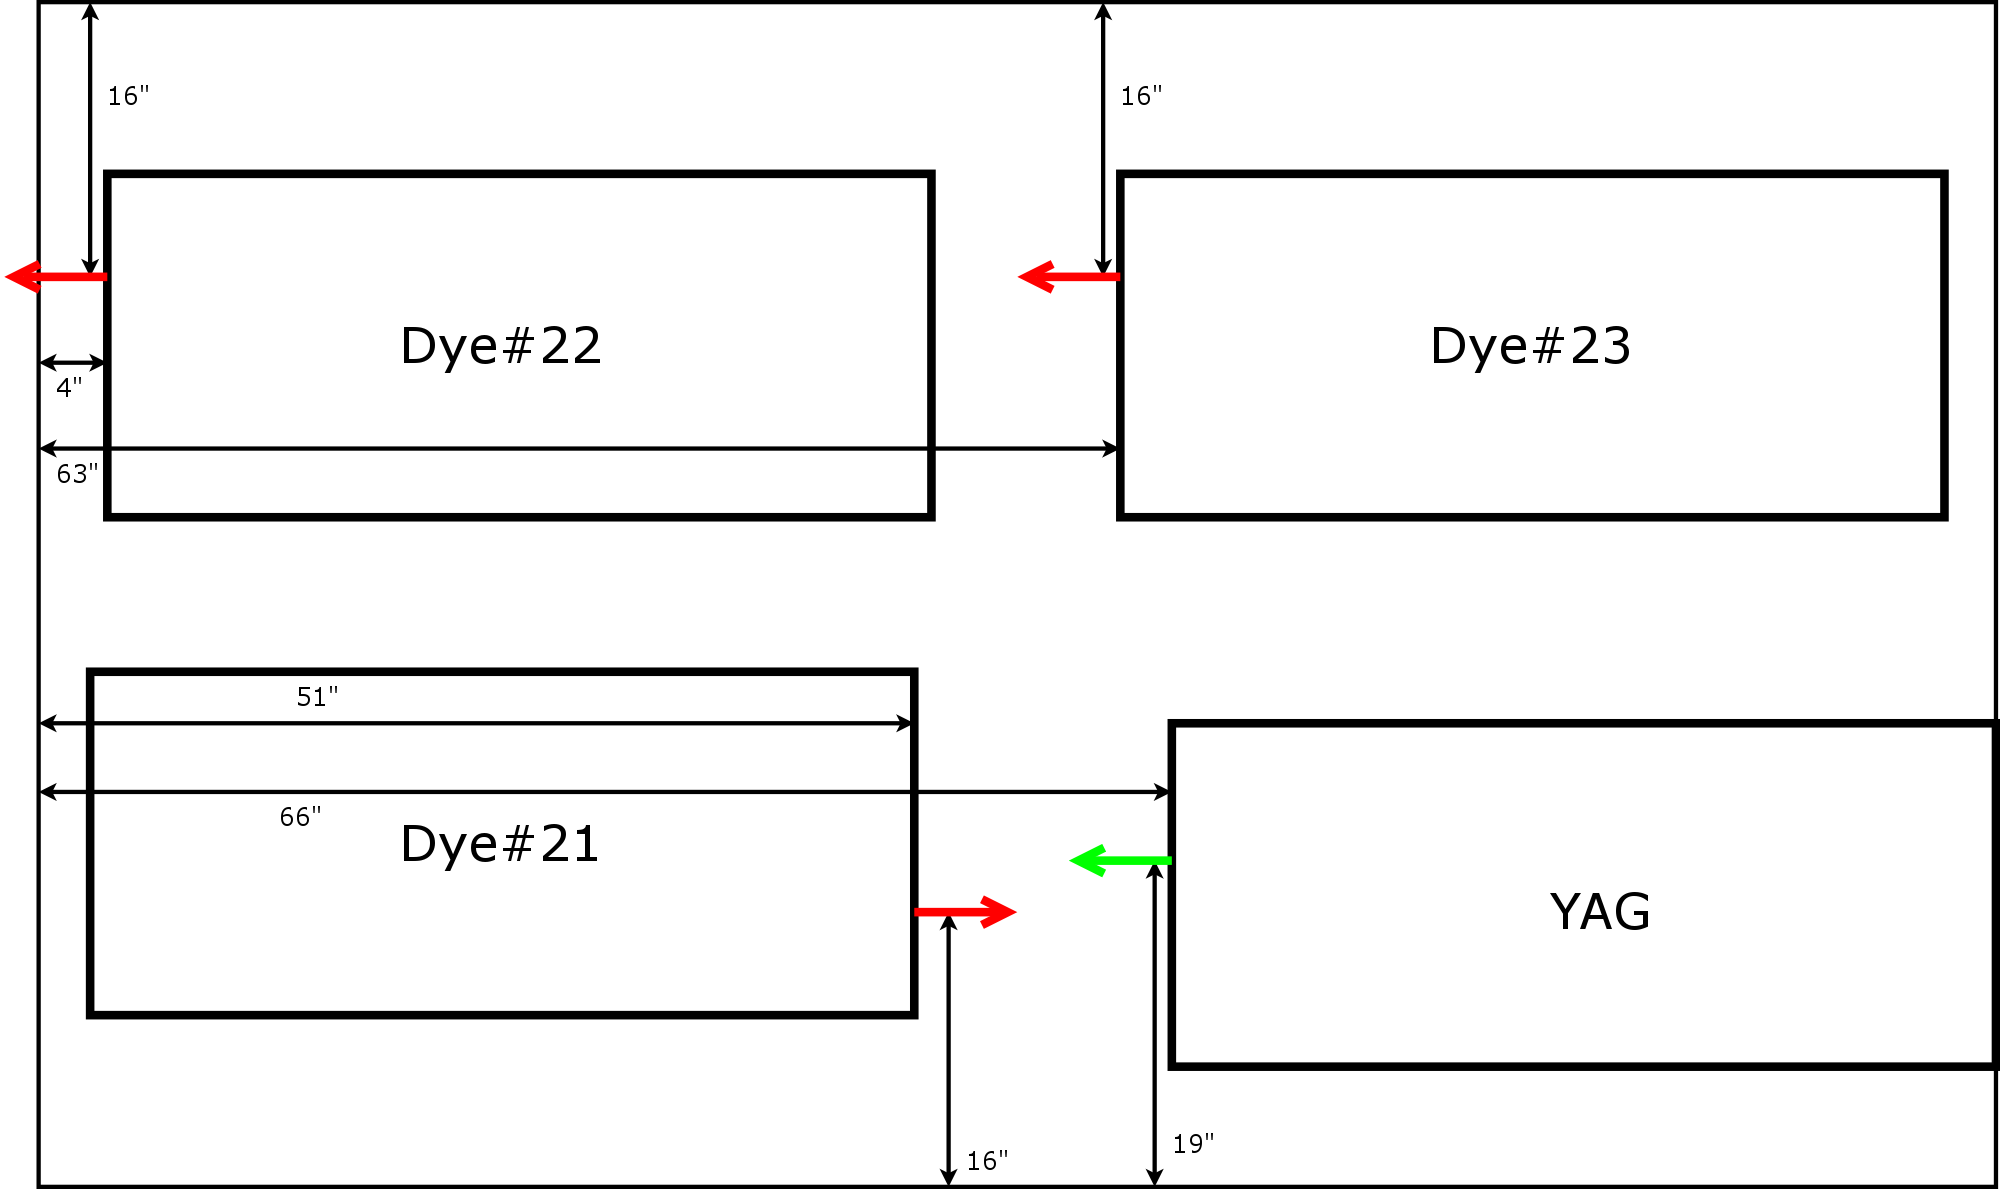
\includegraphics[width=7.75in]
{laser_positions/laser_positions.png}\\
\caption[Laser positions on dye laser table]{Laser positions on dye laser table. The outside border of the diagram (i.e., the reference edge for all dimensions) is the line defined by the last column (or row) of 1/4-20 tapped holes on the optical bench (NOT the actual edge of the table).}
\label{laser_positions}
\end{sidewaysfigure} 
%----------------------------------------------------------------------------
%----------------------------------------------------------------------------
%----------------------------------------------------------------------------



%----------------------------------------------------------------------------

The output from the Nd:YAG is split into three equal parts and sent to the input ports of each dye laser. First the beam is sent though a beam splitter that transmits two thirds of the incident beam power and reflects the remaining third. The transmitted beam is then sent though a beam splitter that transmits half and reflects half the incident beam power. In this way, we pump each dye laser with equal power allowing the most flexibility when exploring different pulse sequences. See figure \ref{YAG_positions}
%----------------------------------------------------------------------------
% YAG_positions.tex
% by Troy Hix, May 2005
%----------------------------------------------------------------------------
\begin{sidewaysfigure}
\center
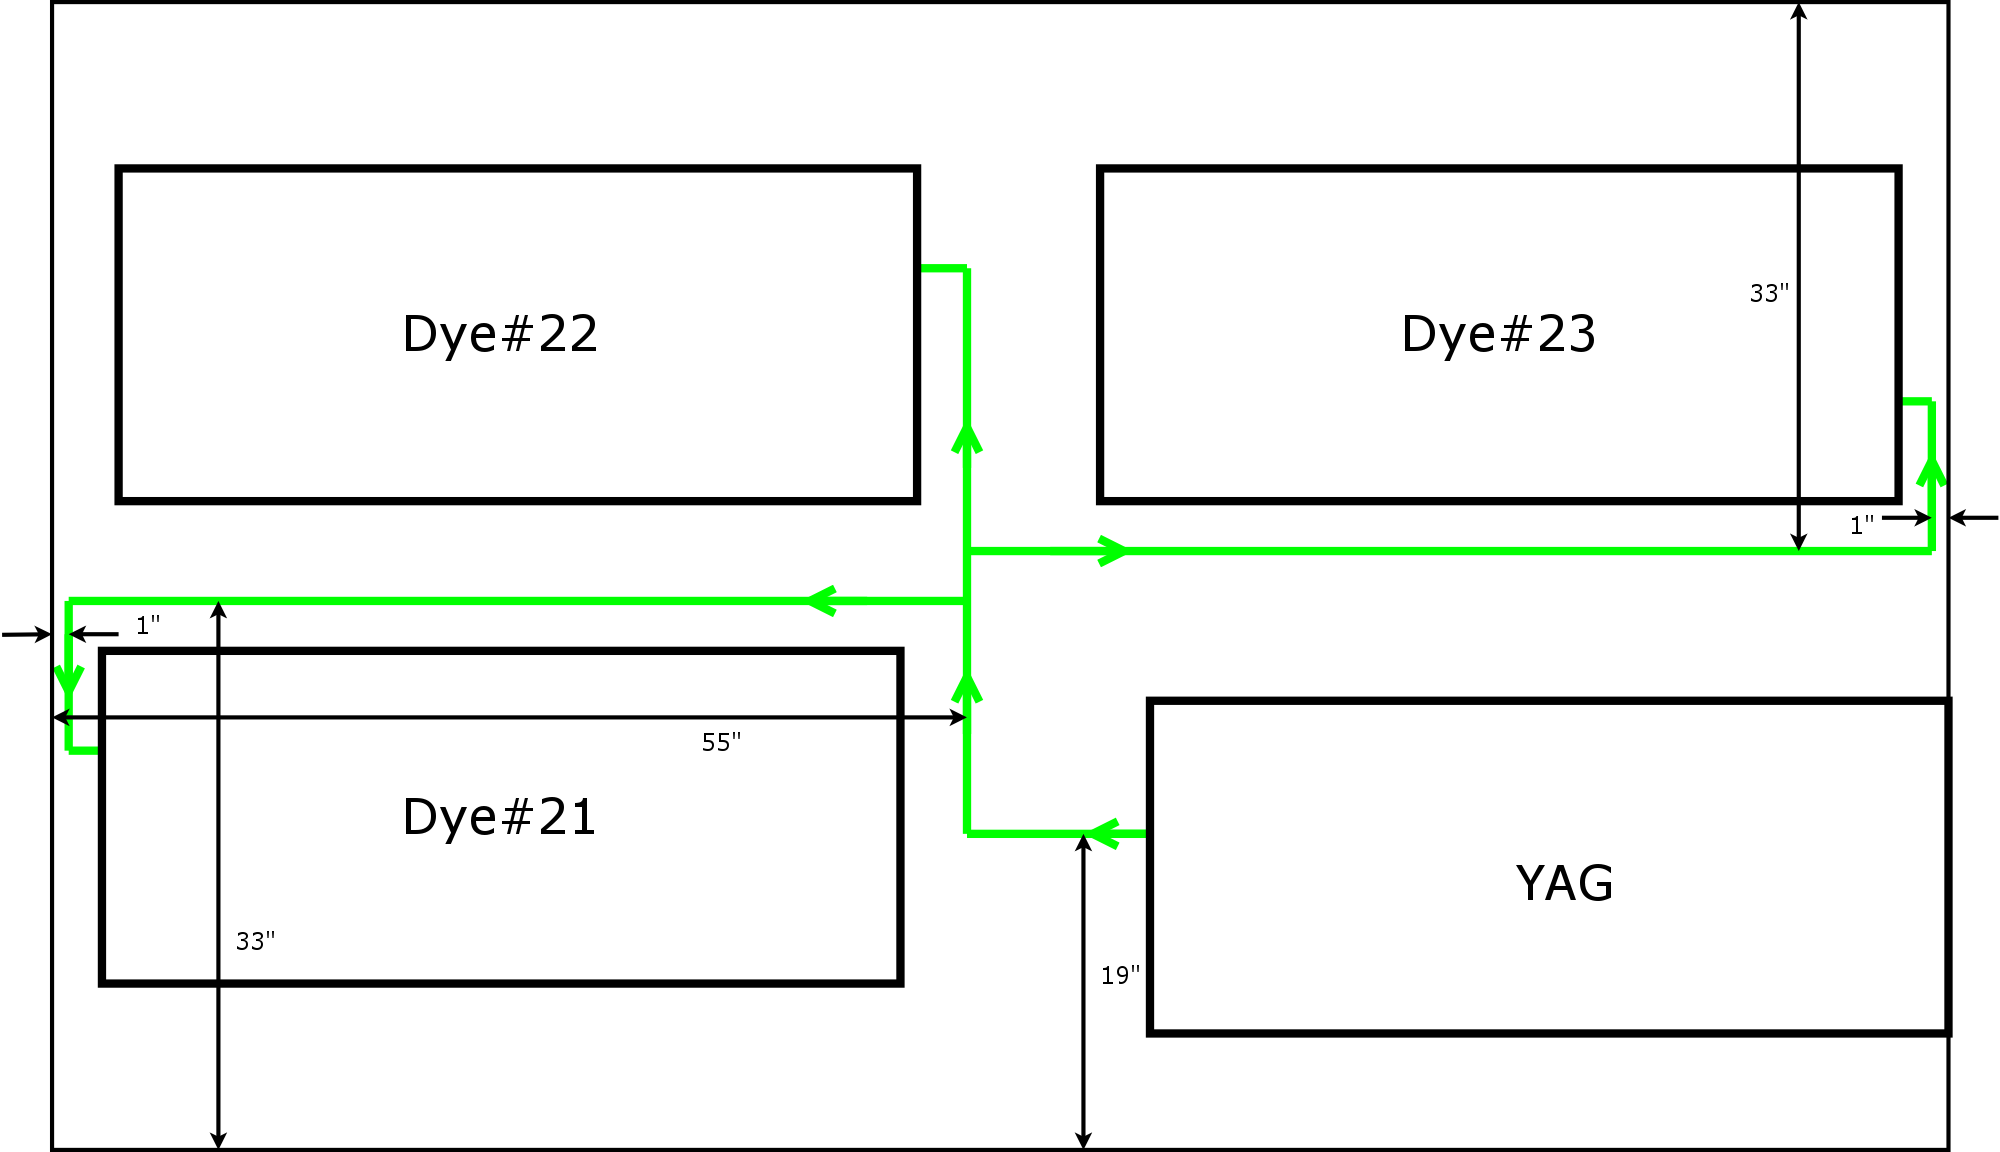
\includegraphics[width=7.75in]
{YAG_positions/YAG_positions.png}\\
\caption{YAG beam positions}
\label{YAG_positions}
\end{sidewaysfigure} 
%----------------------------------------------------------------------------
%----------------------------------------------------------------------------
%----------------------------------------------------------------------------



%----------------------------------------------------------------------------

The output from each dye laser is conditioned with respect to polarization and amplitude before it leaves the dye laser table. This is mainly for safety reasons, but also has the added advantage of localizing the Pockels cell system, along with its associated fast high voltage electronics, far from the data acquisition region of the experiment. The relative delay between each beam is adjusted on the dye laser table to allow for a convenient beam line on the next two tables. See figure \ref{dye_positions}.
%----------------------------------------------------------------------------
% dye_positions.tex
% by Troy Hix, May 2005
%----------------------------------------------------------------------------
\begin{sidewaysfigure}
\center
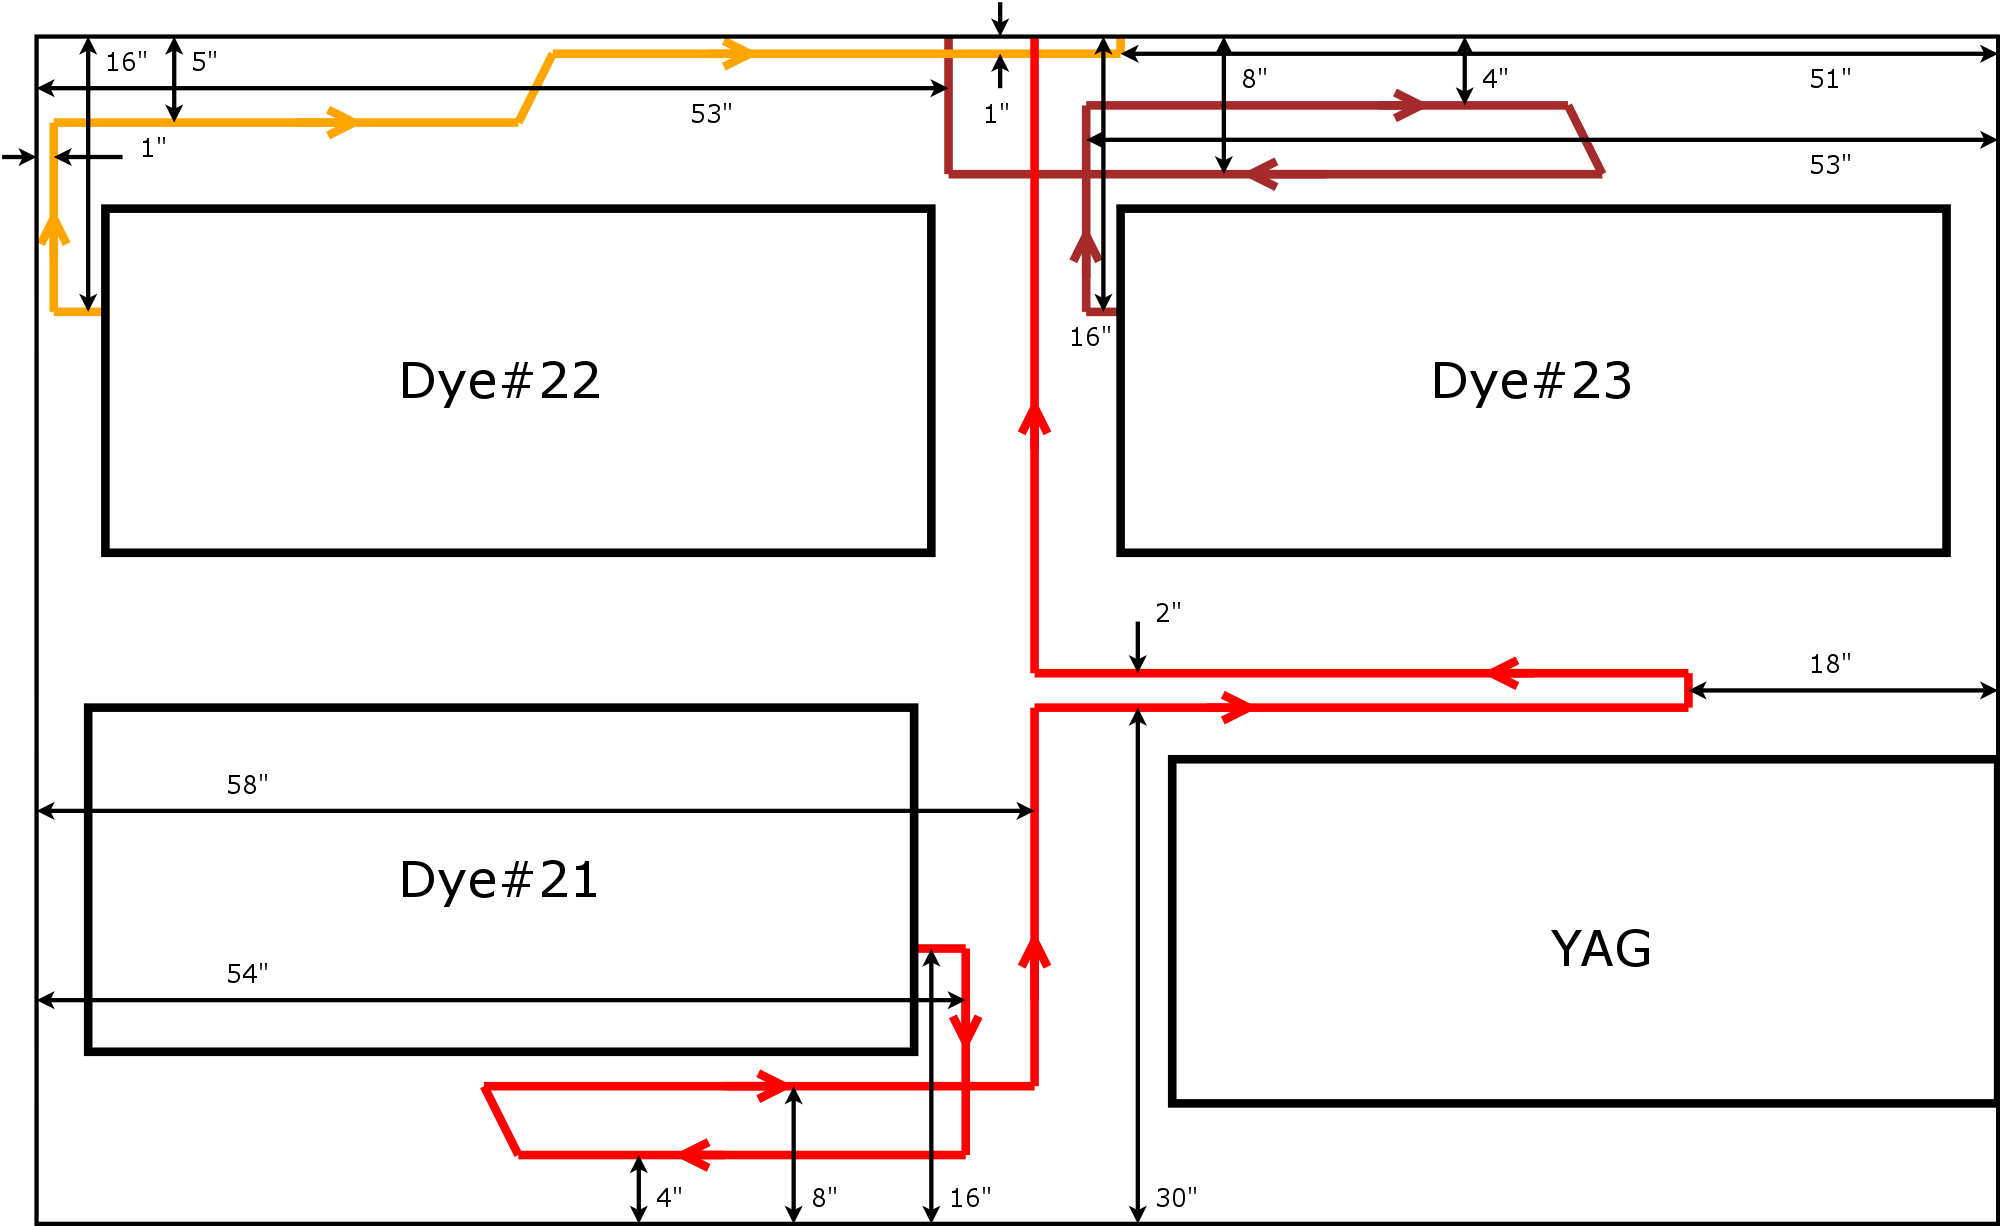
\includegraphics[width=7.75in]
{dye_positions/dye_positions.png}\\
\caption{Dye beam positions}
\label{dye_positions}
\end{sidewaysfigure} 
%----------------------------------------------------------------------------
%----------------------------------------------------------------------------
%----------------------------------------------------------------------------



%----------------------------------------------------------------------------

The Pockels cell system consists of a pile-of-plates polarizer, a Pockels cell, then a Brewster plate. The output of the pile-of-plates will be highly polarized in the horizontal direction. When switched, the Pockels cell will rotate this horizontal polarization toward the vertical by a specified amount. The Brewster plate will then output a sample of the vertical component of this beam. In this way we produce a vertically polarized output beam with continuously selectable pulse energy. See figure \ref{dye_mileposts}
%----------------------------------------------------------------------------
% dye_table_mileposts.tex
% by Troy Hix, May 2005
%----------------------------------------------------------------------------
\begin{sidewaysfigure}
\center
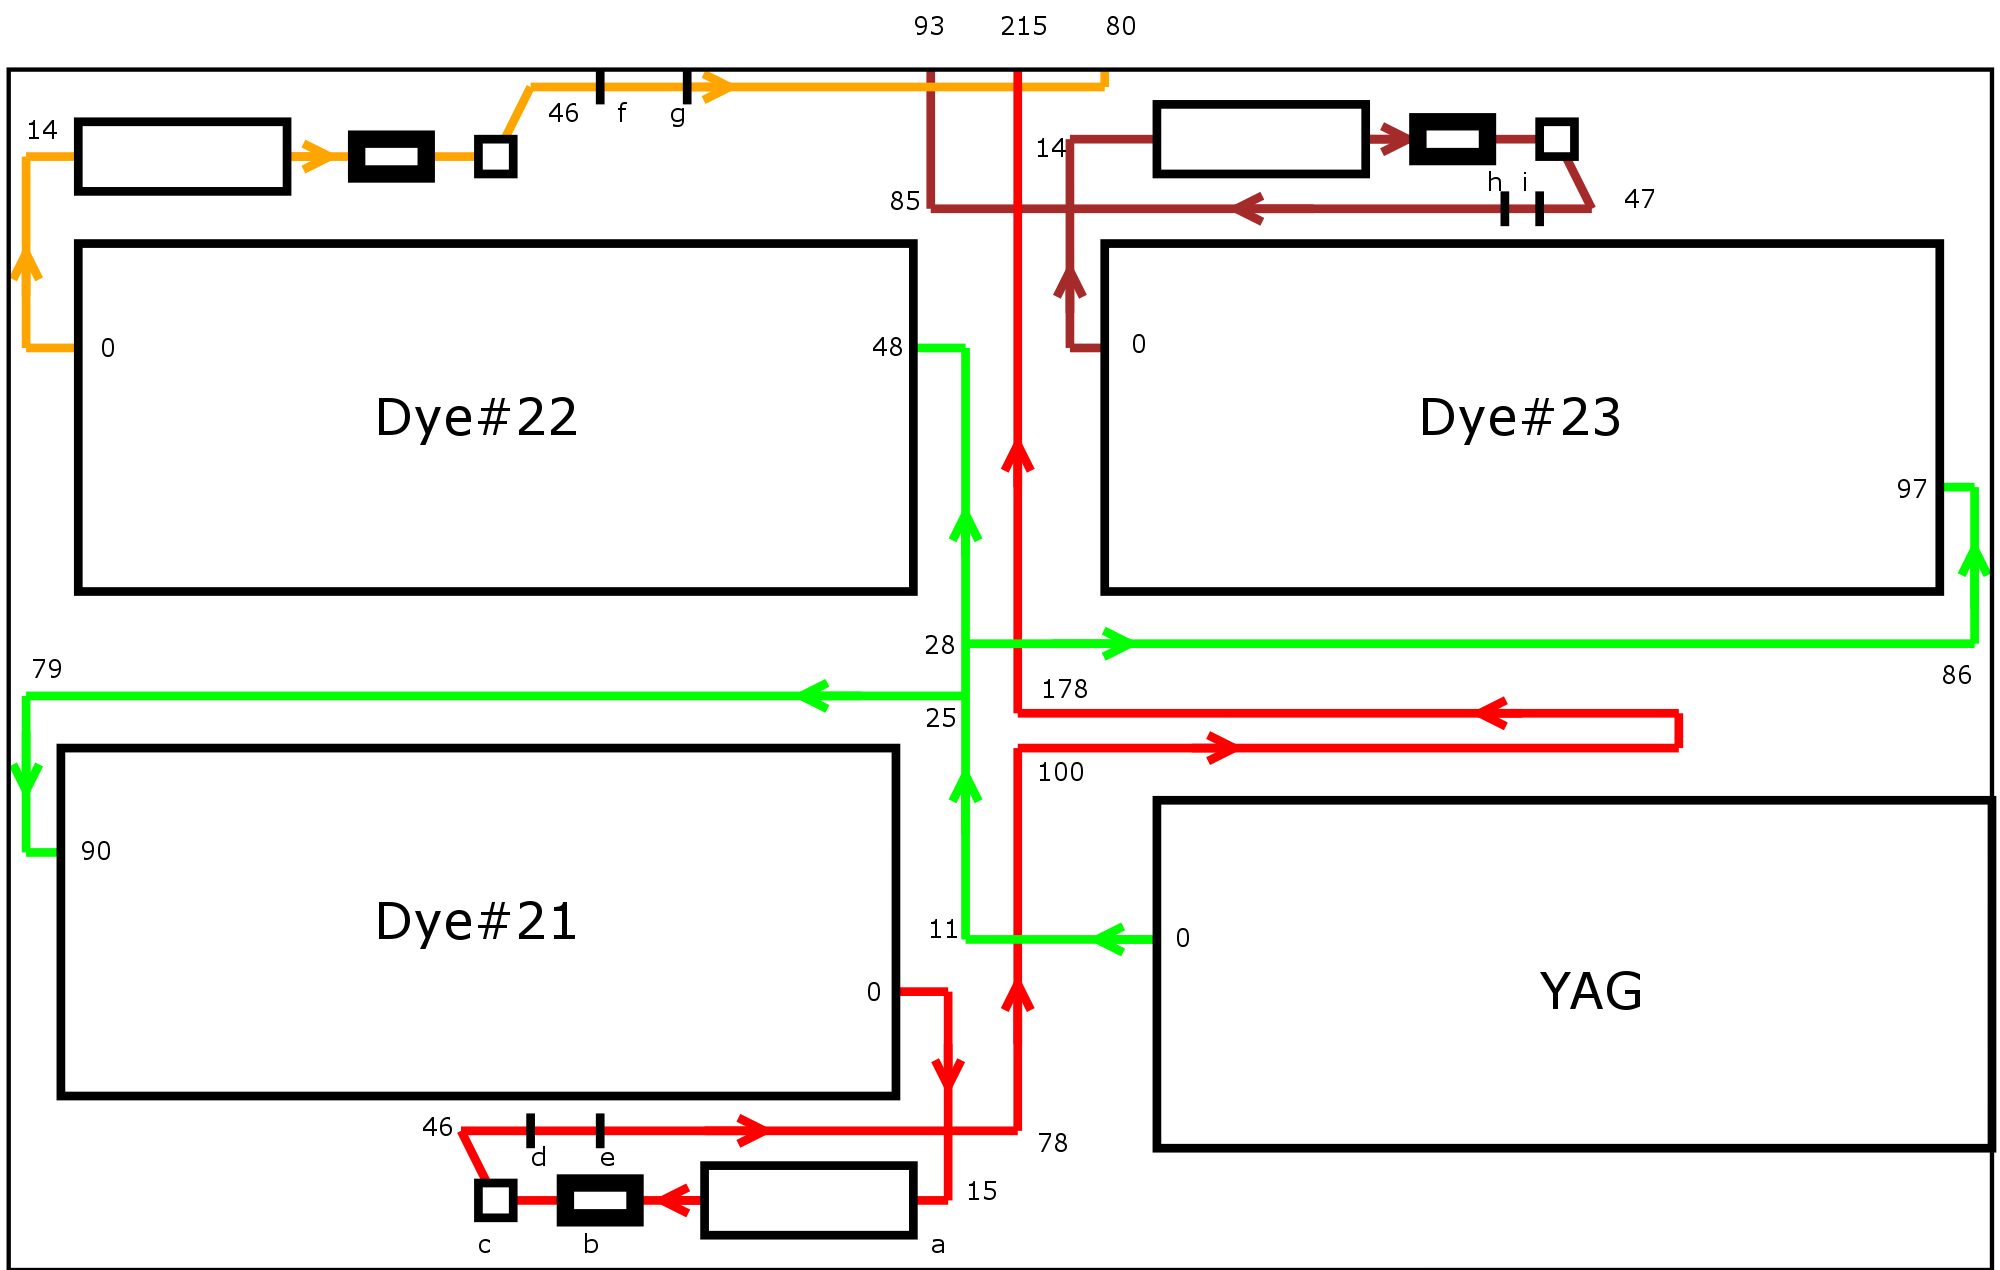
\includegraphics[width=7.75in]
{dye_mileposts/dye_mileposts.png}
\caption[Beam mileposts and optics on the dye laser table]{Beam mileposts and optics on the dye laser table. the mileposts along each beam line is given in inches. Optic (a) is a pile-of-plates polarizer; (b) Pockels cell, (c) Brewster plate, (d) +1 m lens at mile post 50, (e) -1 m lens at milepost 54, (f) +1 m lens at milepost 50, (g) -1 m lens at milepost 55, (h) +1 m lens at milepost 50, (i) -1 m lens at milepost 52.5.}
\label{dye_mileposts}
\end{sidewaysfigure} 
%----------------------------------------------------------------------------
%----------------------------------------------------------------------------
%----------------------------------------------------------------------------



%----------------------------------------------------------------------------
%----------------------------------------------------------------------------
%----------------------------------------------------------------------------
%----------------------------------------------------------------------------
%----------------------------------------------------------------------------

%----------------------------------------------------------------------------
\subsection{Beam conditioning table}
%----------------------------------------------------------------------------
%----------------------------------------------------------------------------
On the conditioning table we delay and spatially filter the three dye laser beams. The delay line is a rail with a sliding ``car'' which the user moves by hand. With the beam line folded four times, we can achieve delays of $\pm$ 8 ns using a 4 foot rail. It will only be necessary to delay two of the beams (dye lasers \#22 and \#23) to generate arbitrary pulse sequences with internal delays less than 8 ns. After the beams are synchronized, we spatially filter each beam using a pinhole. The filter consists of a focusing lens, high damage threshold pinhole, and a collimating lens to capture the usable portion of the pinhole output. See figure \ref{conditioning_table}.
%----------------------------------------------------------------------------
% conditioning_table.tex
% by Troy Hix, May 2005
%----------------------------------------------------------------------------
\begin{sidewaysfigure}
\center
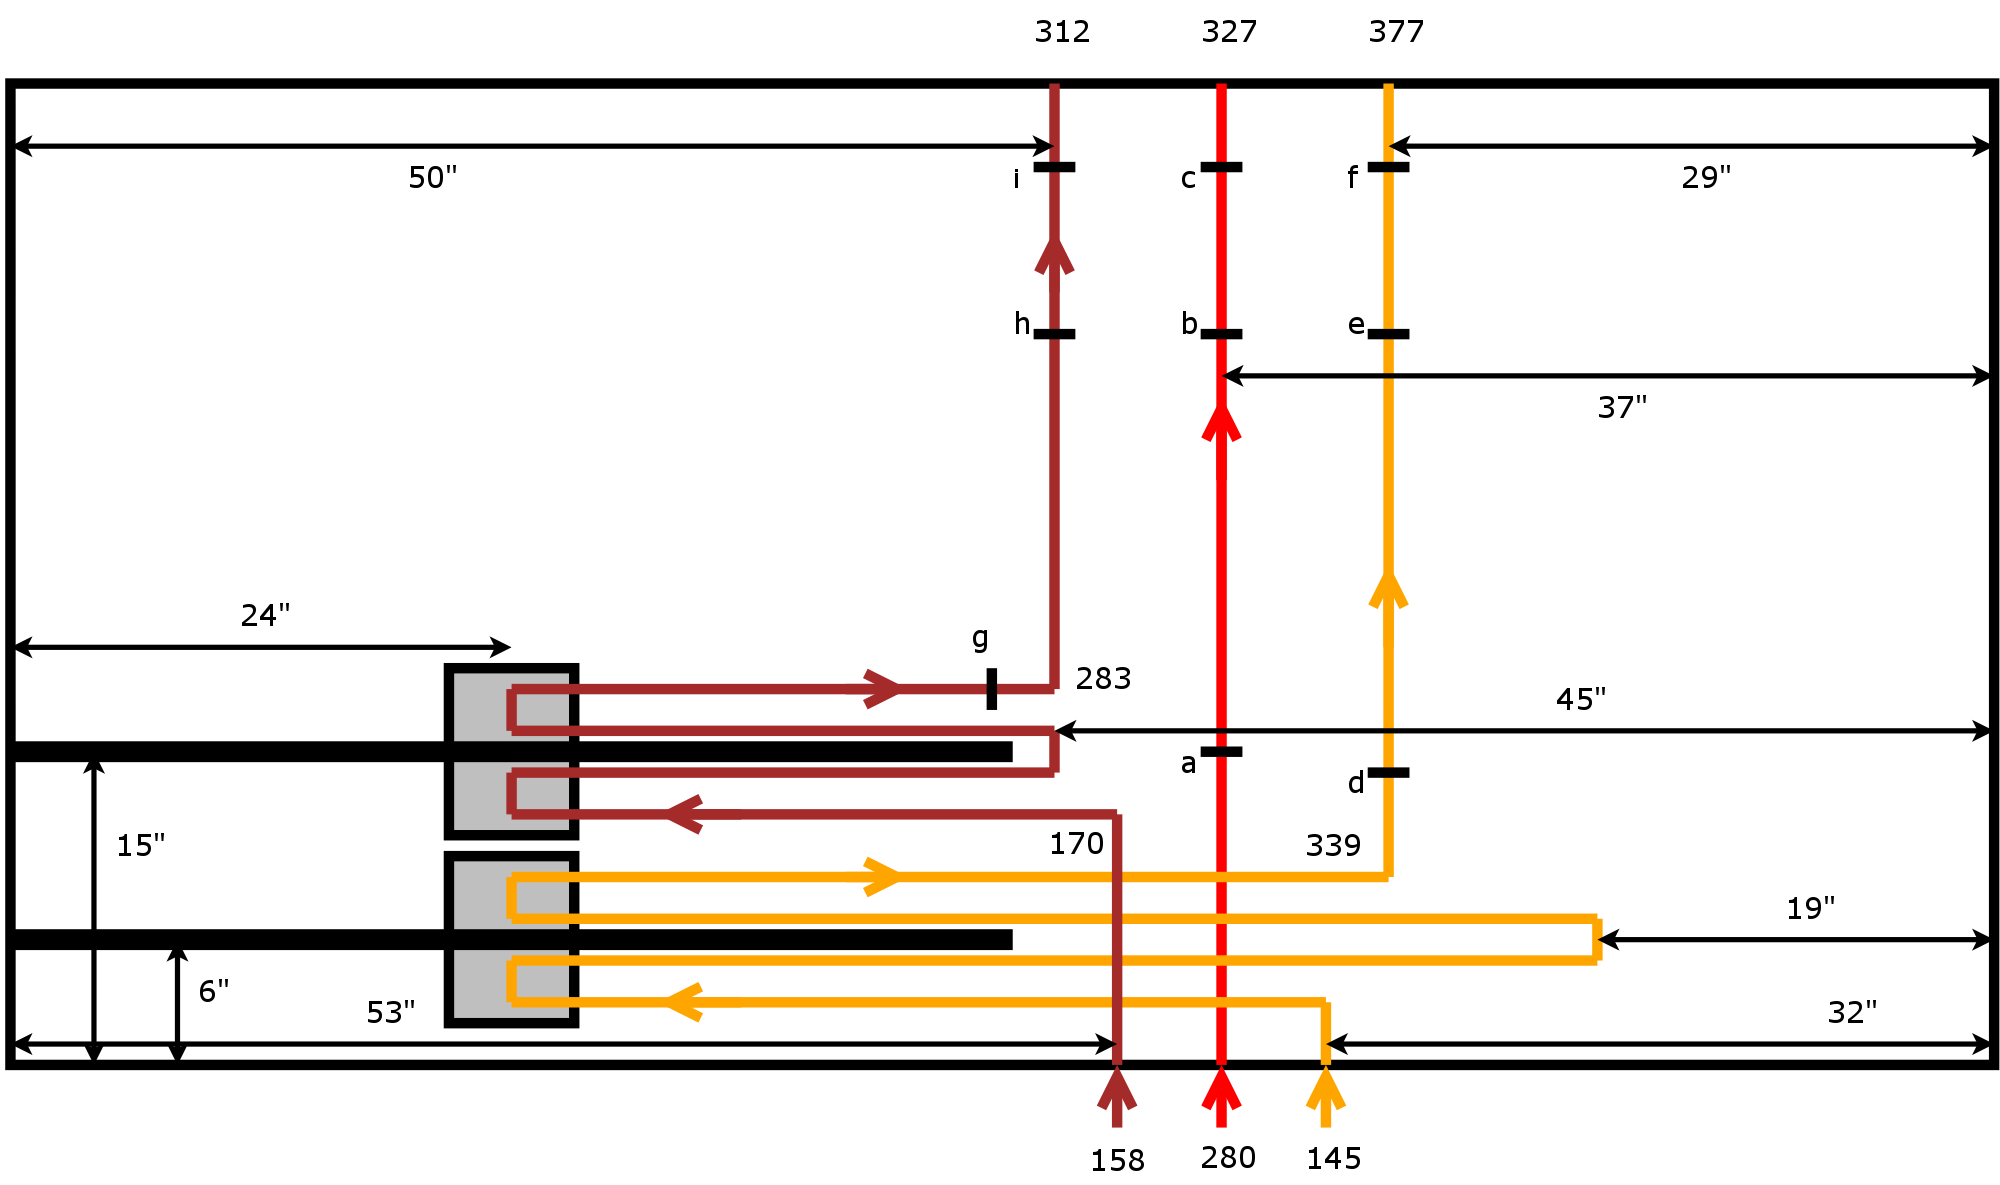
\includegraphics[width=7.75in]
{conditioning_table/conditioning_table.png}\\
\caption[Beam conditioning table]{Beam conditioning table. (a) is a +0.5 m lens at milepost 295, (b) is a pinhole at milepost 315.3, (c) is a +0.2 m lens at milepost 323.2, (d) is a +0.5 m lens at milepost 344, (e) is a pinhole at milepost 364.7, (f) is a +0.2 m lens at milepost 372.5, (g) is a +0.5 m lens at milepost 280, (h) is a pinhole at milepost 300.3, and (i) is a +0.2 m lens at milepost 308.2. The delay lines are shown as horizontal black bars; the delay ``cars'' (in the zero delay position) are shown as gray rectangles.}
\label{conditioning_table}
\end{sidewaysfigure} 
%----------------------------------------------------------------------------
%----------------------------------------------------------------------------
%----------------------------------------------------------------------------



%----------------------------------------------------------------------------
%----------------------------------------------------------------------------
%----------------------------------------------------------------------------
%----------------------------------------------------------------------------
%----------------------------------------------------------------------------

%----------------------------------------------------------------------------
\subsection{Interaction table}
%----------------------------------------------------------------------------
%----------------------------------------------------------------------------
The interaction table begins with the final stage of conditioning: spectral filtering. The spectral filter is an etalon with a FSR $<$ 3GHz (to prevent aliasing) and mode widths ranging from 100 MHz (for long pulse experiments) to 552 MHz (for short pulse experiments). The beam line presented here assumes planar etalons - some redesign will be required if confocal etalons are used. See figure \ref{interaction_mileposts}.
%----------------------------------------------------------------------------
% interaction_table_mileposts.tex
% by Troy Hix, May 2005
%----------------------------------------------------------------------------
\begin{sidewaysfigure}
\center
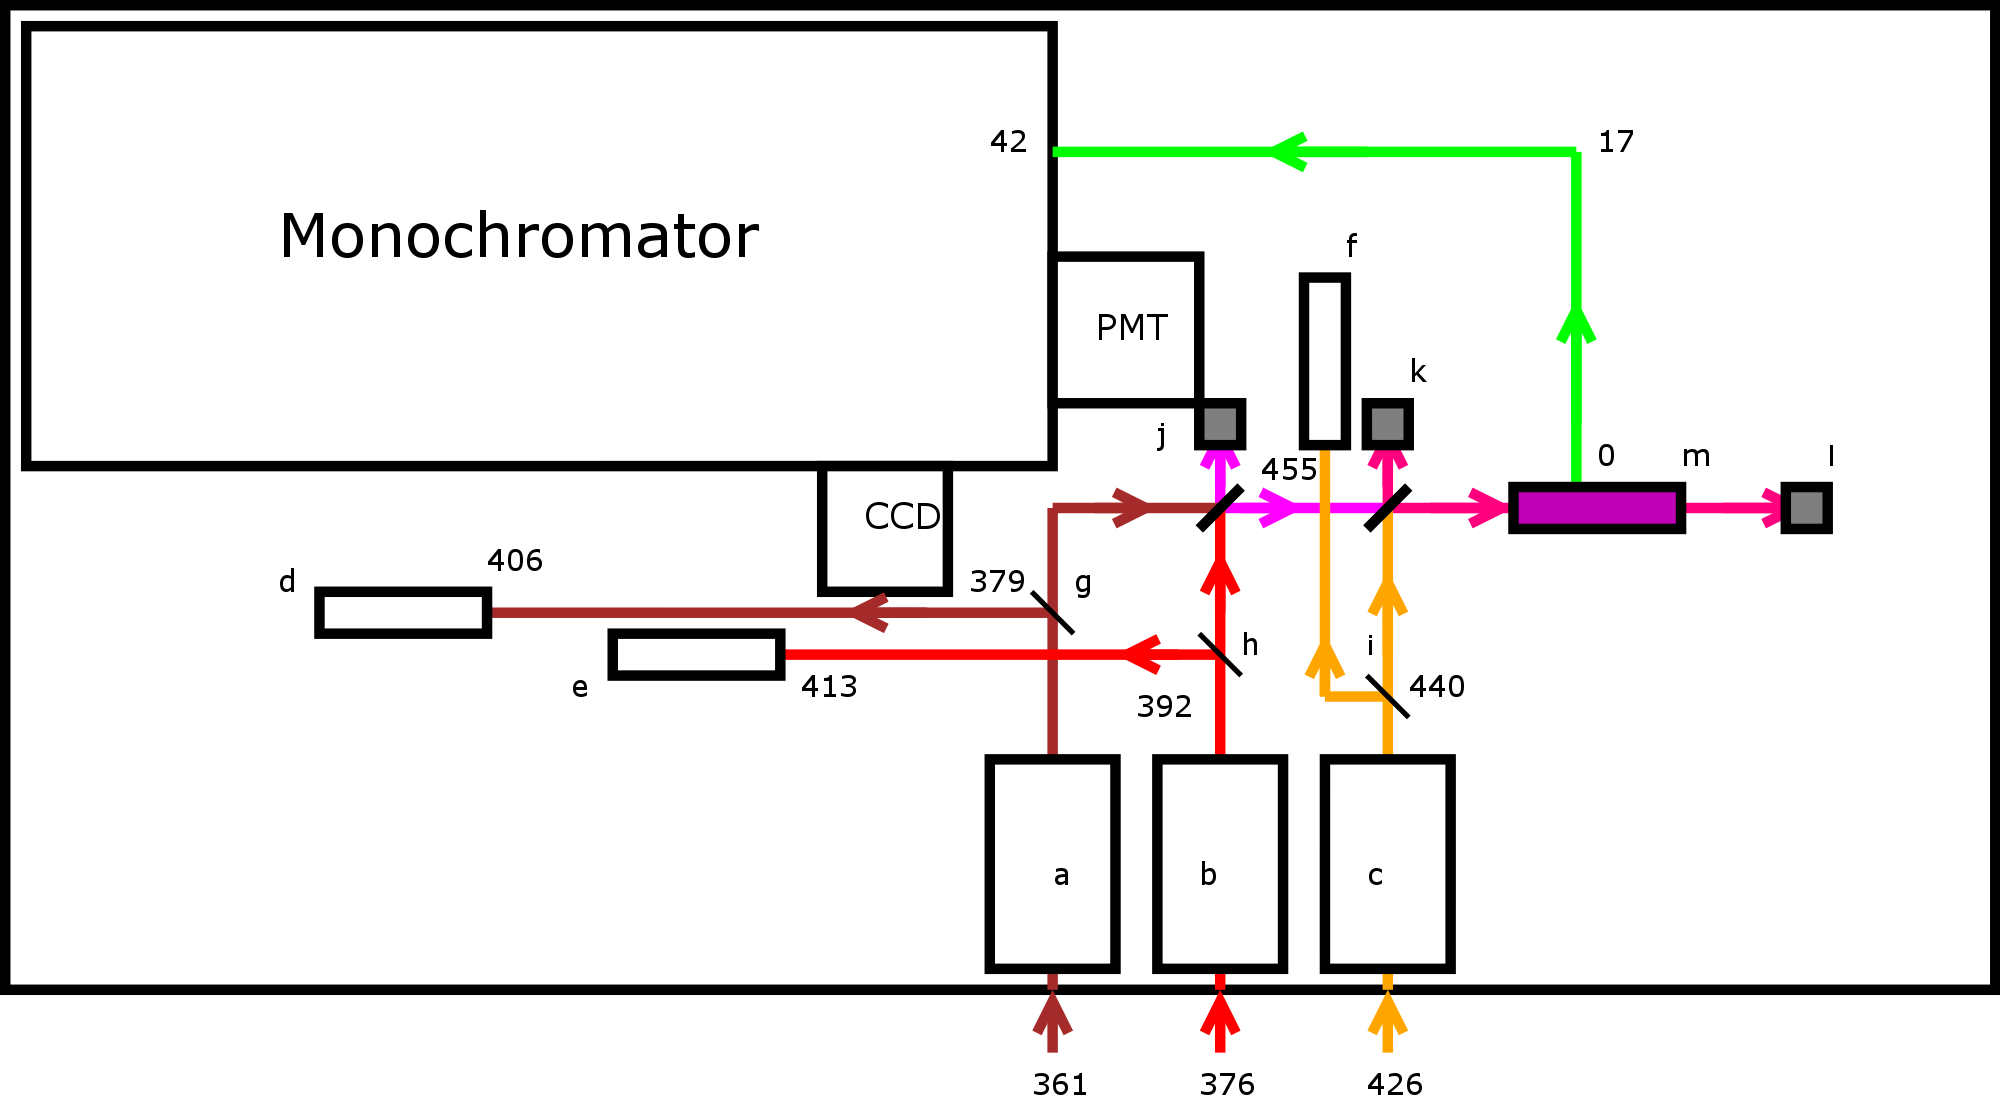
\includegraphics[width=7.75in]
{interaction_mileposts/interaction_mileposts.png}
\caption[Interaction table beam mileposts and optical component labels]{Interaction table beam mileposts and optical component labels. There is a 6X8 inch foot print for the etalons (a), (b), and (c). (d),(e), and (f) are the energy meters and pinholes for each beam. (g) is a pick-off placed at milepost 379 along the beam from dye laser \#23 - similarly for (h) and (i). (j), (k), and (l) are beam dumps and (m) is the iodine cell and its pinhole.}
\label{interaction_mileposts}
\end{sidewaysfigure} 
%----------------------------------------------------------------------------
%----------------------------------------------------------------------------
%----------------------------------------------------------------------------



%----------------------------------------------------------------------------

The three dye laser beams are then mixed using beam splitters. Once the beam are collinear, they are incident upon a pinhole placed just upstream from the iodine cell. Pick-offs are placed before the beams splitters to sample each input beam. Energy detectors are placed downstream from the pick-offs so that they are at the same beam milepost as the iodine cell. Duplicate pinholes are placed upstream from each detector; identical to the iodine cell's pinhole. Figure \ref{interaction_positions} shows the beam positions required.
%----------------------------------------------------------------------------
% interaction_table_positions.tex
% by Troy Hix, May 2005
%----------------------------------------------------------------------------
\begin{sidewaysfigure}
\center
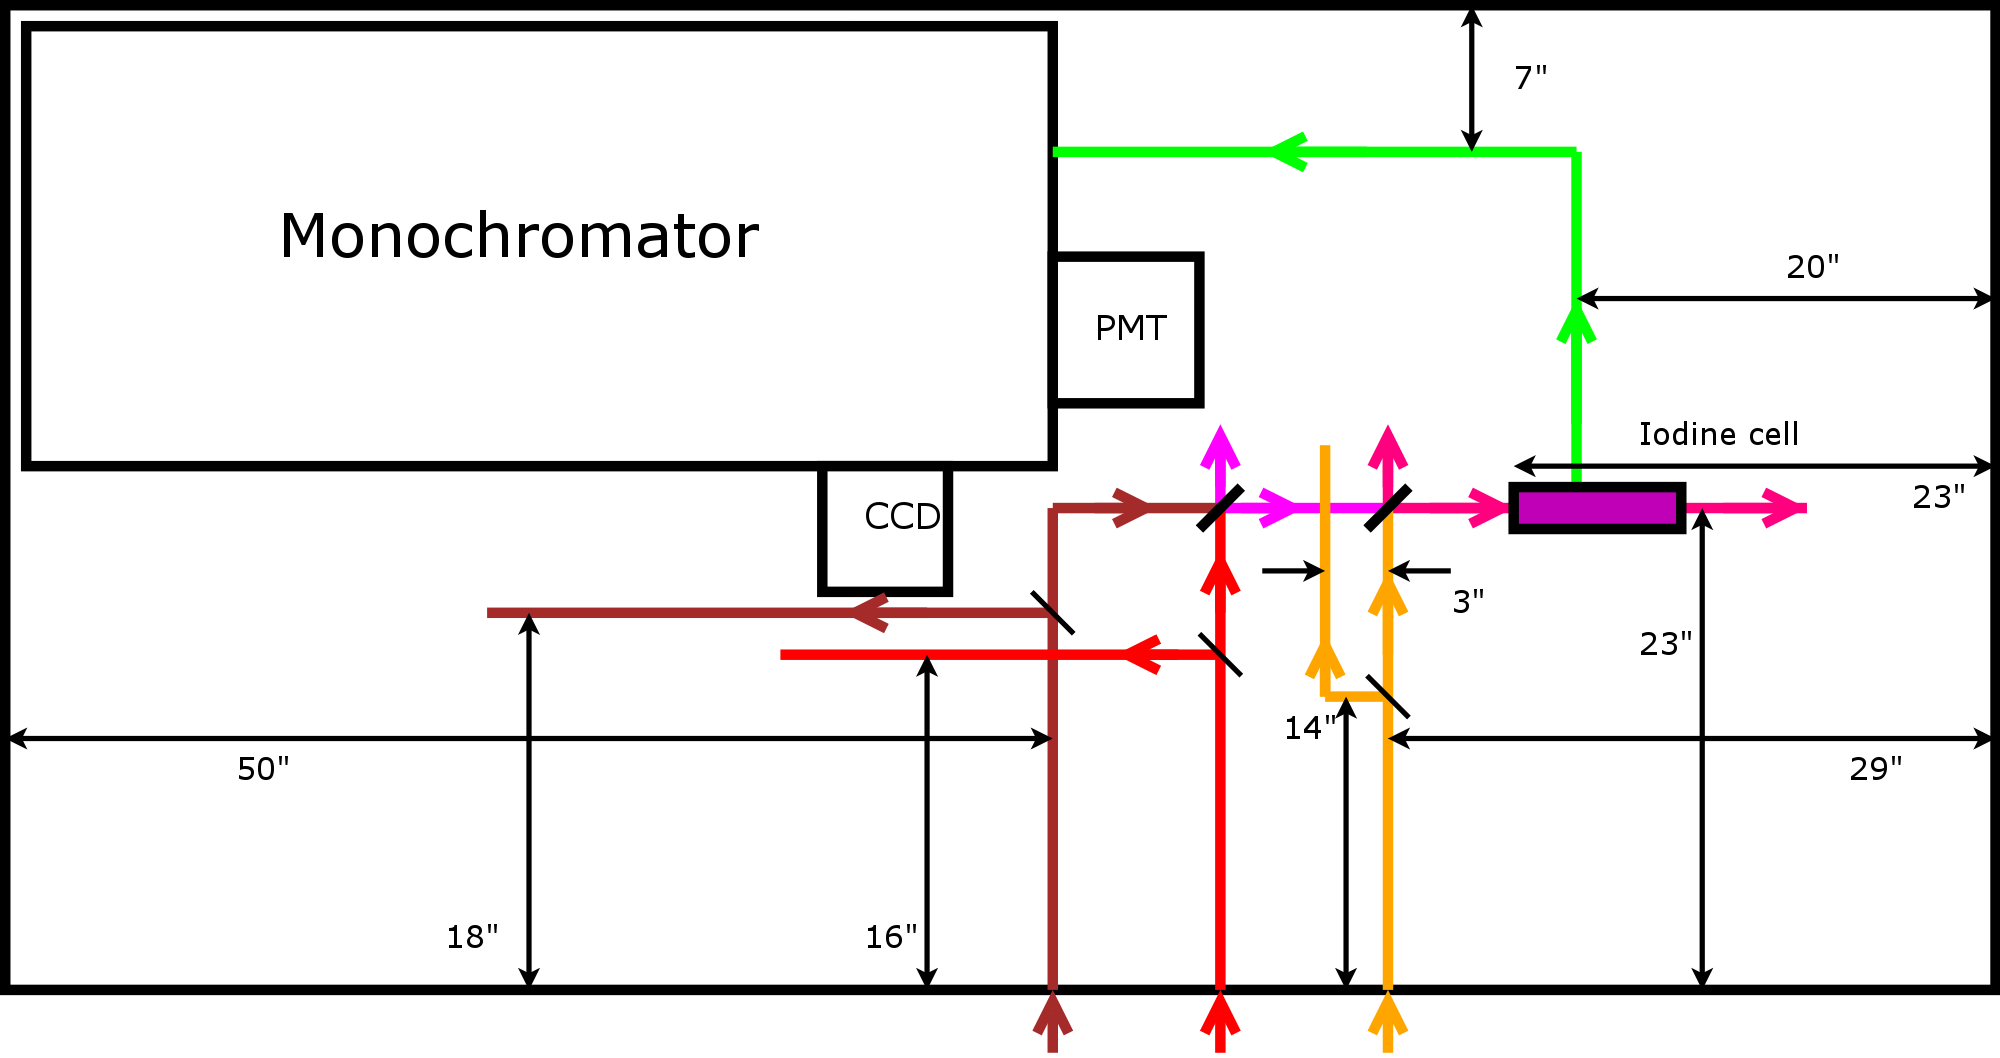
\includegraphics[width=7.75in]
{interaction_positions/interaction_positions.png}
\caption[Interaction table beam positions]{Interaction table beam positions. The mixed beams are shown in light pink and dark pink, the green beam is the fluorescence signal.}
\label{interaction_positions}
\end{sidewaysfigure} 
%----------------------------------------------------------------------------
%----------------------------------------------------------------------------
%----------------------------------------------------------------------------



%----------------------------------------------------------------------------


In figure \ref{interaction_mileposts} we see that the beam from dye laser \#21 traveled 413 inches to reach the energy detector labeled (e) in the figure. This is the same distance the beam travels to reach the iodine cell labeled (m). If we add the distance the YAG beam traveled to pump dye laser \#21 we obtain 503 inches. It can be shown using figures \ref{dye_mileposts} and \ref{interaction_mileposts} that the other two dye lasers have this same sum. Thus, assuming the path lengths inside each dye laser is the same, we conclude the three pulses arrive at the iodine cell (and the energy detectors) simultaneously.
%----------------------------------------------------------------------------
% dye_table_mileposts.tex
% by Troy Hix, May 2005
%----------------------------------------------------------------------------
\begin{sidewaysfigure}
\center
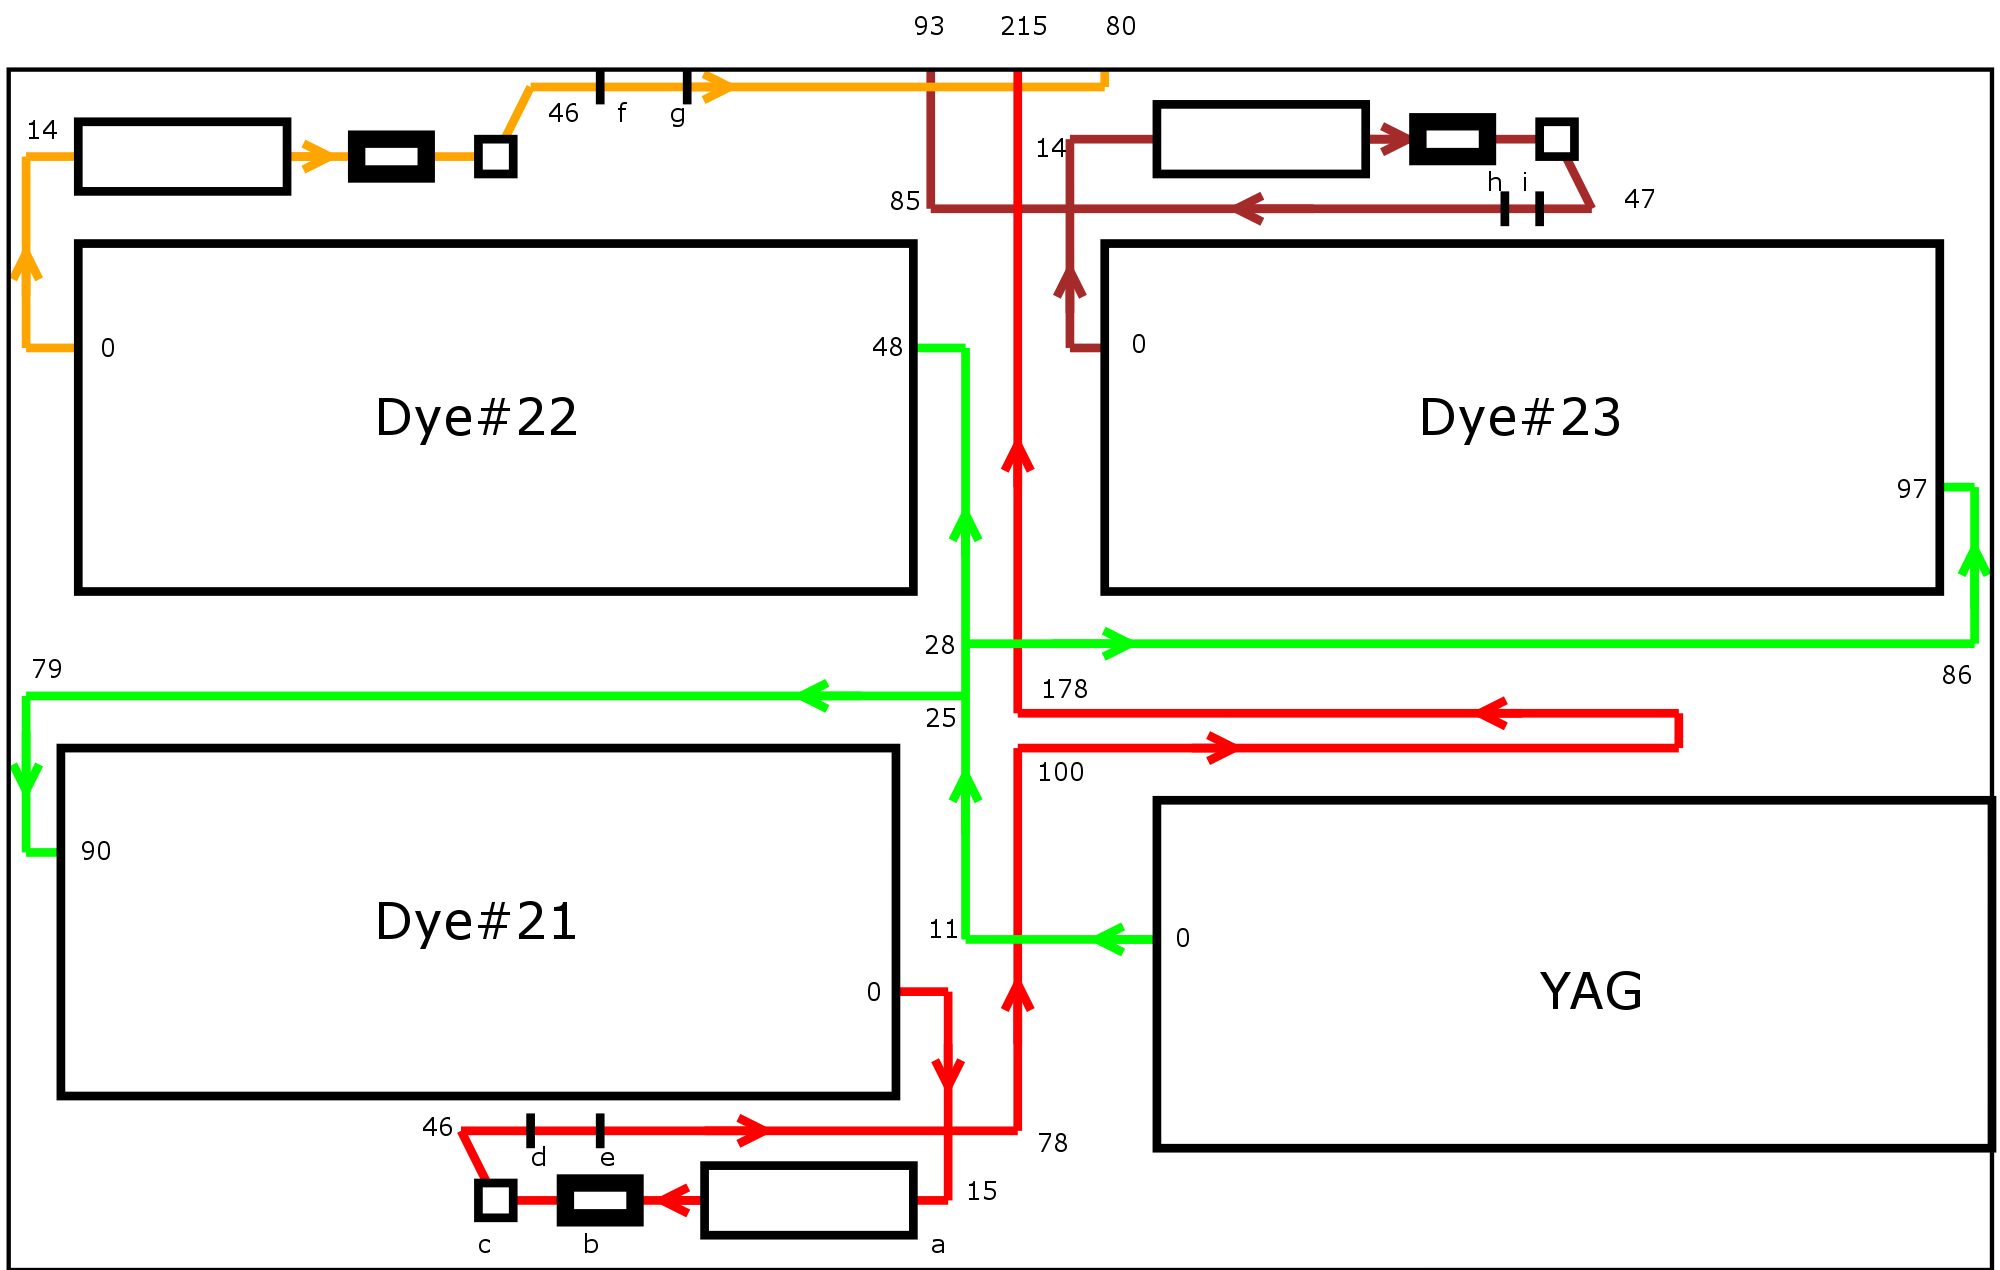
\includegraphics[width=7.75in]
{dye_mileposts/dye_mileposts.png}
\caption[Beam mileposts and optics on the dye laser table]{Beam mileposts and optics on the dye laser table. the mileposts along each beam line is given in inches. Optic (a) is a pile-of-plates polarizer; (b) Pockels cell, (c) Brewster plate, (d) +1 m lens at mile post 50, (e) -1 m lens at milepost 54, (f) +1 m lens at milepost 50, (g) -1 m lens at milepost 55, (h) +1 m lens at milepost 50, (i) -1 m lens at milepost 52.5.}
\label{dye_mileposts}
\end{sidewaysfigure} 
%----------------------------------------------------------------------------
%----------------------------------------------------------------------------
%----------------------------------------------------------------------------



%----------------------------------------------------------------------------
%----------------------------------------------------------------------------
%----------------------------------------------------------------------------
%----------------------------------------------------------------------------
%----------------------------------------------------------------------------

%----------------------------------------------------------------------------
%----------------------------------------------------------------------------
\section{Filters}
There are three filters under consideration: a temporal shaper, a spatial filter, and a band pass spectral filter. The filter with the most development history is the temporal shaper: the Pockels cell. The pinhole is analyzed here in terms of its effectiveness as a spatial filter for high peak power pulsed control experiments. A fundamental limitation on the transmitted power of etalon type filters is parameterized -- this brings into question the rationale for using etalons when beam energy is important to the experiment. Finally we present the results of a test of a confocal etalon purchased for evaluation purposes.
%----------------------------------------------------------------------------
\subsection{Pockels cells DC test}
%----------------------------------------------------------------------------
\label{DC test section}
%----------------------------------------------------------------------------
%----------------------------------------------------------------------------
%----------------------------------------------------------------------------
%bb defines the bounding box for the pdf
%viewport defines the area of the pdf used
%in sidewaysfigure the last entry in bb moves the caption toward/away the pic
%in sidewaysfigure the second entry in bb moves the pic toward/away the caption
%----------------------------------------------------------------------------
\begin{figure}
\scalebox{0.8}[0.8]{
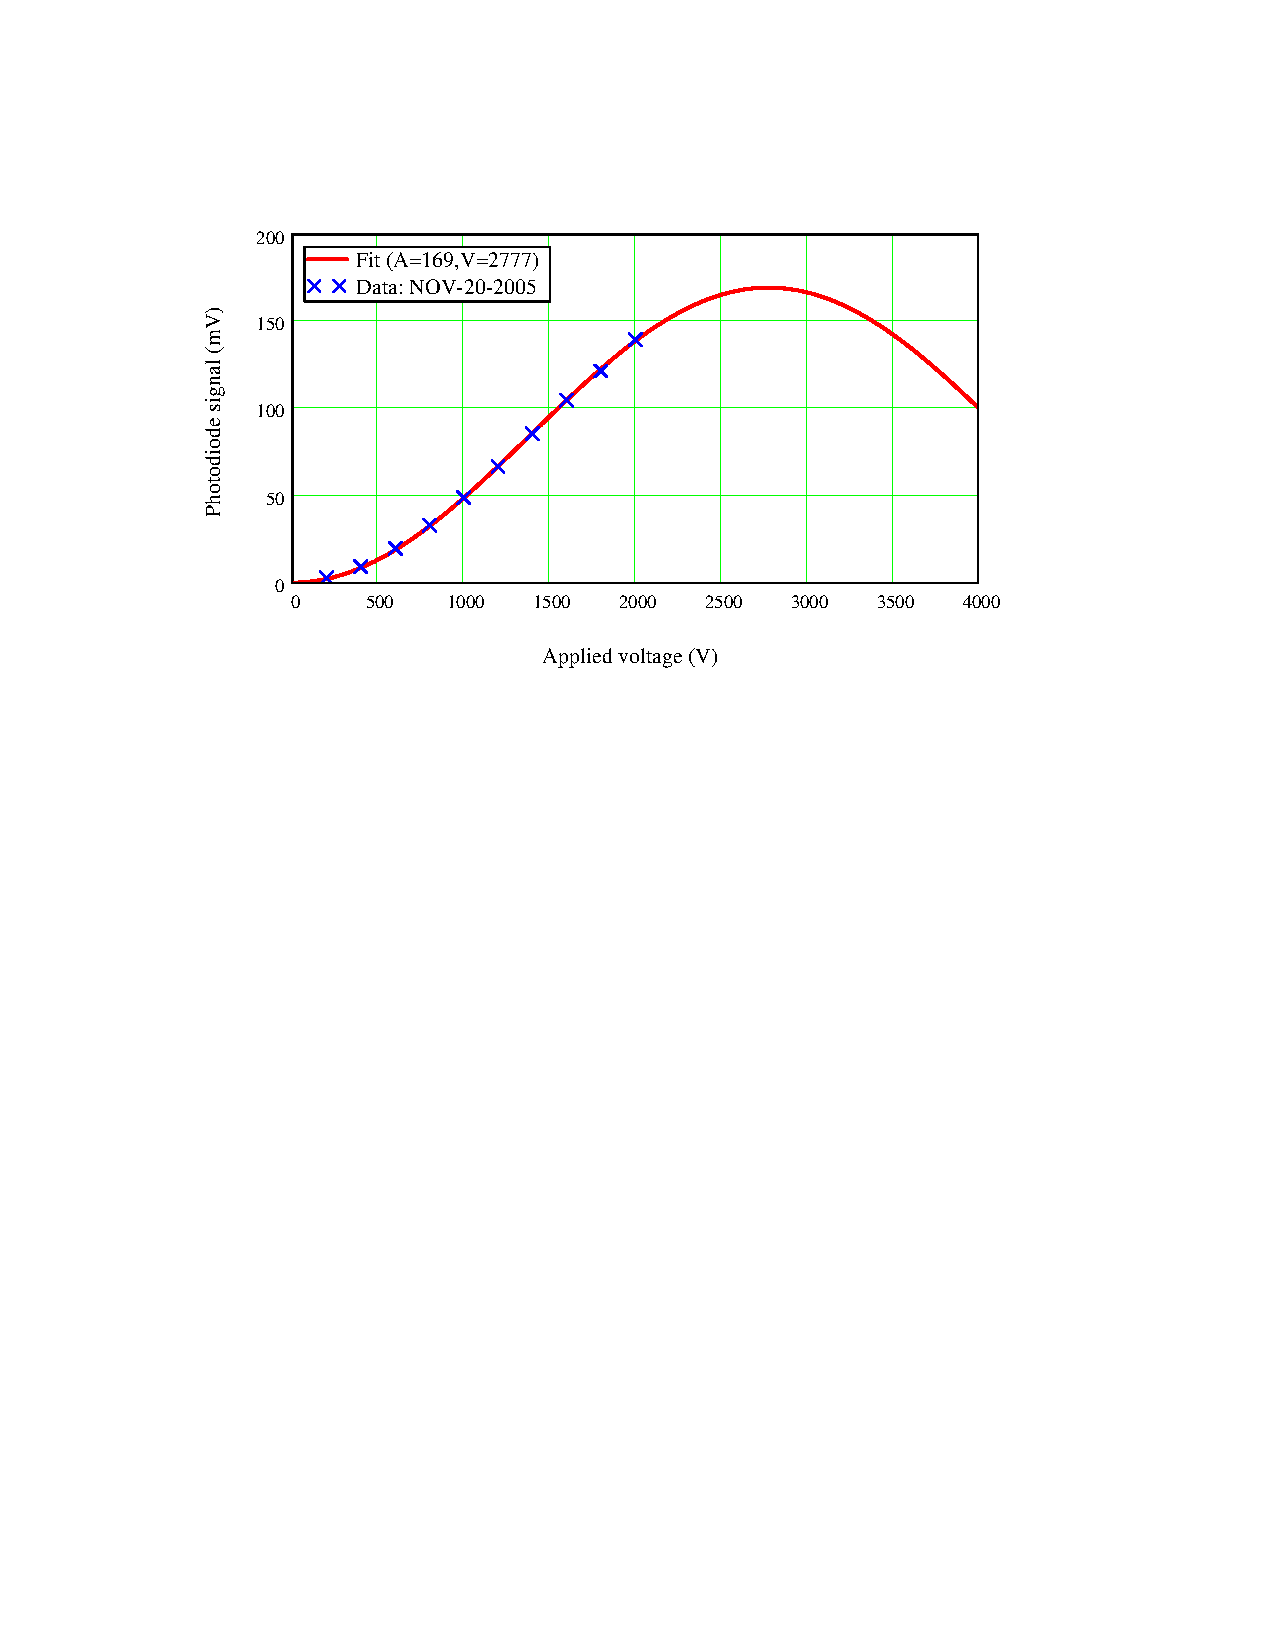
\includegraphics[bb=30 467 481 706]
{fit_628/fit_628.pdf}
}
\caption[DC test of 628nm coated Pockels cell]{DC test of 628nm coated Pockels cell. A base line photodiode reading (with the crossed polarizers and Pockels cell removed) was not recorded for these data; however, we expect the efficiency to be better than the green case in Figure \ref{fit_532} since the laser wavelength of 633nm is closer to AR coating wavelength.}
\label{fit_628}
\end{figure}
%----------------------------------------------------------------------------

%----------------------------------------------------------------------------
%bb defines the bounding box for the pdf
%viewport defines the area of the pdf used
%in sidewaysfigure the last entry in bb moves the caption toward/away the pic
%in sidewaysfigure the second entry in bb moves the pic toward/away the caption
%----------------------------------------------------------------------------
\begin{figure}
\scalebox{0.8}[0.8]{
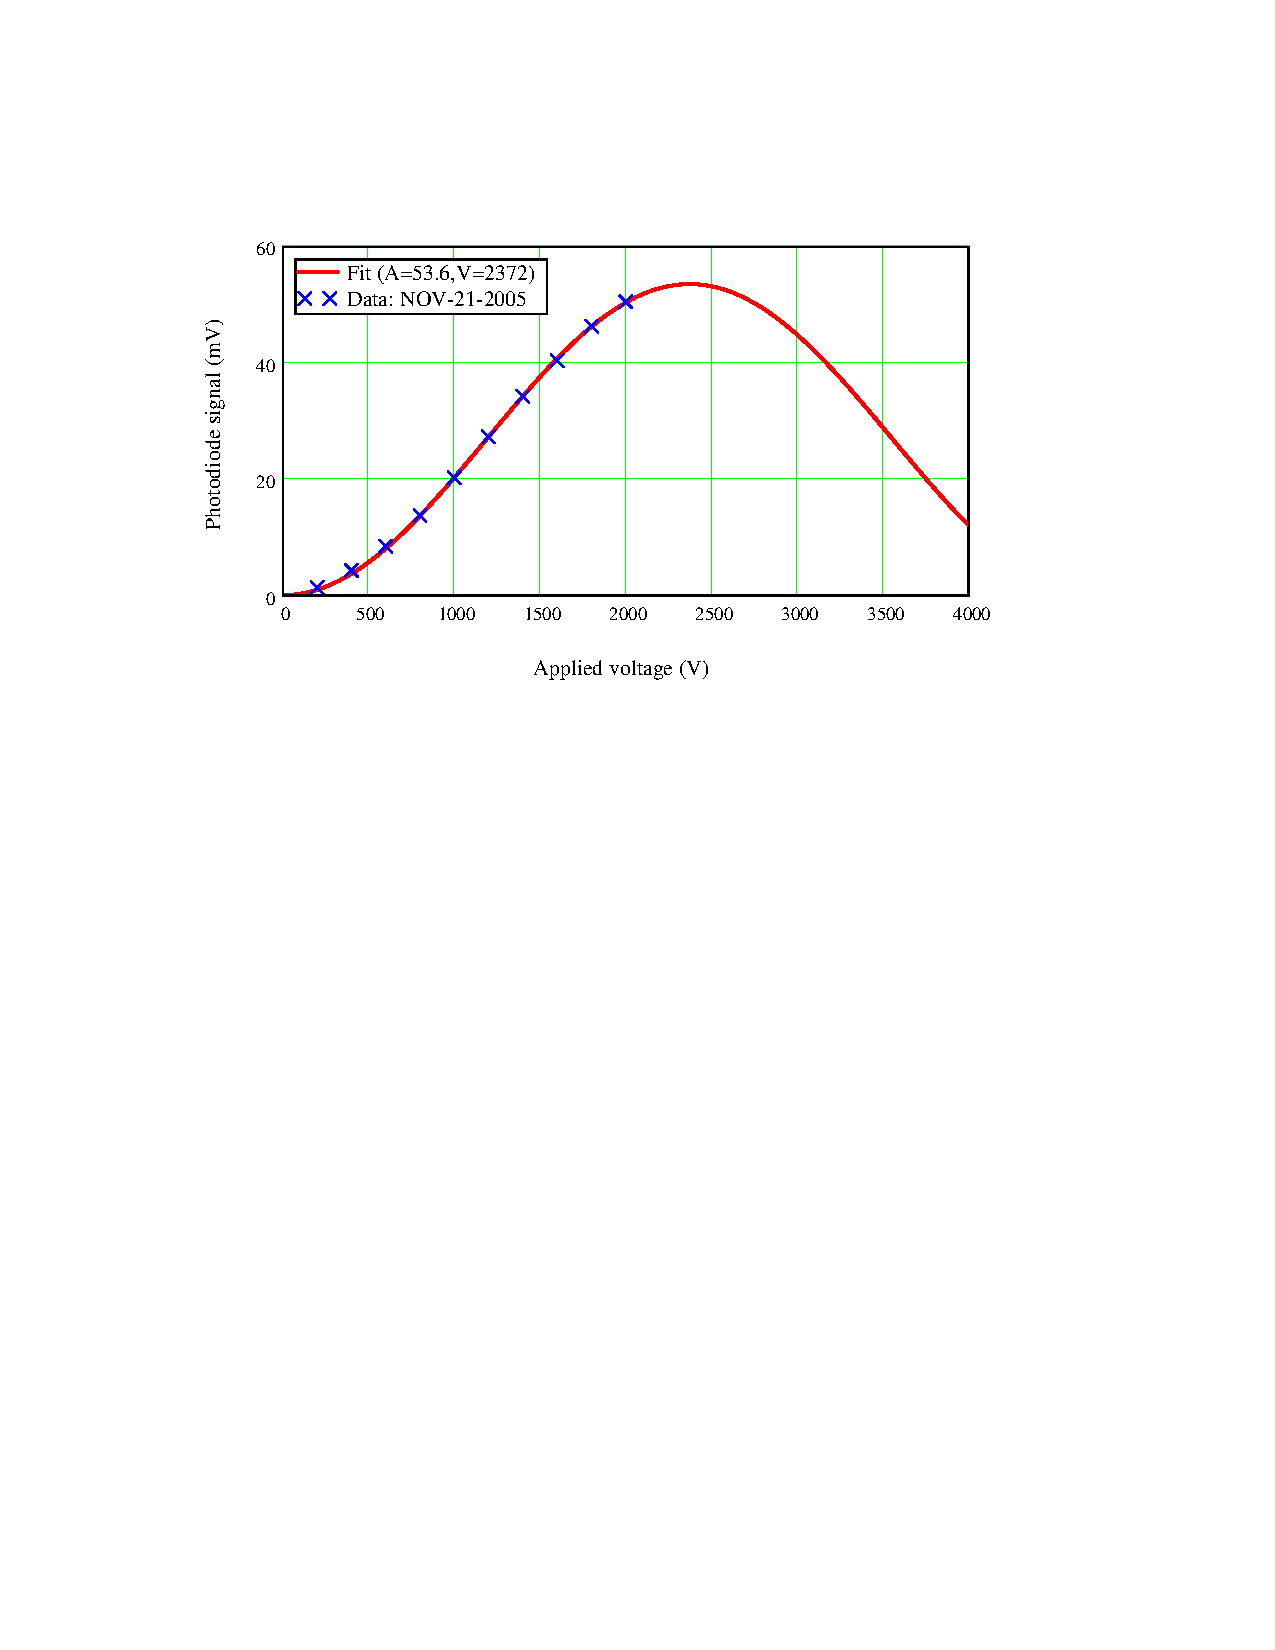
\includegraphics[bb=30 460 481 706]
{fit_532/fit_532.pdf}
}
\caption[DC test of 532nm coated Pockels cell]{DC test of 532nm coated Pockels cell. Since the photodiode signal is 76 mV with the crossed polarizers and Pockels cell removed, the fit value for A (53.6 mV) implies an efficiency of $e \sim 70\%$. Some of the attenuation may be due to the fact the laser wavelength of 543nm is different than the AR coating wavelength. The polarizers will also contribute to the attenuation factor for the system.}
\label{fit_532}
\end{figure}
%----------------------------------------------------------------------------

%----------------------------------------------------------------------------
Here we describe a test to determine a basic performance parameter of the Pockels cell: the applied voltage at which a beam passing through the cell will experience a 90 degree polarization rotation. By placing the Pockels cell between two crossed polarizers (10LP-VIS, Newport), the complete system (crossed polarizers and Pockels cell) becomes a light gate with respect to the applied voltage. If the cell is in a state where the polarization is not rotated, then light cannot pass through the system. However, if the Pockels cell rotates the beam polarization, significant power can begin to pass through the system. Maximum transmission occurs when the beam polarization is rotated 90$^\circ$. Specifically \cite{Saleh:1991a},
\begin{equation}
P_{out}
(V_a)
=
P_{in} e
\sin^2
\left(
\frac{\pi V_a}{2 V}
\right)
\label{power transmitted}
\end{equation}
where ${P_{out}}$ is the power downstream the system, $P_{in}$ is the power incident the system, $e$ is the efficiency of the system, $V_a$ is the applied voltage, and $V$ is the voltage at which maximum transmission occurs.

The mount for the Pockels cell provides delicate adjustment of the cell's orientation and clearance for the high voltage connectors. The Pockels cell is sensitive to yaw and pitch, requiring fine adjustment, while coarse adjustment of the roll angle and translation was sufficient. A transformer which increases the pulse height by a factor of two is placed close to the Pockels cell. The connection between the Pockels cell and the transformer is made using short wires about 2'' in length. This connection produces a lot of RF noise when the cell is run at high voltages and needs to be shielded to prevent interference with sensitive instruments. A simple tin foil shell was sufficient.

To determine the voltage at which the plane of polarization of a linearly polarized beam is rotated by 90$^\circ$ when run through the Pockels cell, a Hammarlung DC test power supply was used. A collimated CW green HeNe beam was chopped (50\% duty cycle at 200Hz) and sent through the crossed polarizer/Pockels cell system. A large area photodiode (Thorlabs PDA55) was used to detect the power transmitted through the system. A few ND filters were placed upstream the photodiode to select appropriate power levels for the diode. The output of the DC power supply was directly connected to the input terminals of the Pockels cell; thus, when the power supply's foot switch was depressed, the voltage applied to the Pockels cell could be read directly from the meter on the supply. Once the Pockels cell was activated in this manner, the corresponding voltage (representing the power transmitted through the system) from the photodiode could be observed using an oscilloscope.

The input beam to the Pockels cell was vertically polarized, while the Pockels cell was oriented so that the high voltage input terminals were horizontal (the terminals were at the ``9 o'clock'' position when facing downstream toward the cell). DC power supply voltages between 200V and 2000V were used in 200V steps. For each DC voltage applied to the Pockels cell, the corresponding voltage from the photodiode was recorded. A red HeNe was used for the Pockels cell coated for 628nm and a green HeNe was used for the 532nm coating. The data for each cell was fit to Equation \ref{power transmitted}. The coefficient $P_{in} e$ was fit as a single parameter $A$, so the efficiency of the system could be obtained indirectly by measuring the power incident the system and comparing it to the fit parameter $A$. See Figure \ref{fit_628} for the 628nm cell results, and Figure \ref{fit_532} for the 532nm results.

%----------------------------------------------------------------------------
%----------------------------------------------------------------------------

%----------------------------------------------------------------------------
\subsection{Pockels cells minimum pulse length}
%----------------------------------------------------------------------------
\label{Pockels cell pulse section}
%----------------------------------------------------------------------------
%----------------------------------------------------------------------------
%----------------------------------------------------------------------------
%bb defines the bounding box for the pdf
%viewport defines the area of the pdf used
%in sidewaysfigure the last entry in bb moves the caption toward/away the pic
%in sidewaysfigure the second entry in bb moves the pic toward/away the caption
%----------------------------------------------------------------------------
\begin{figure}
\scalebox{0.68}[0.68]{
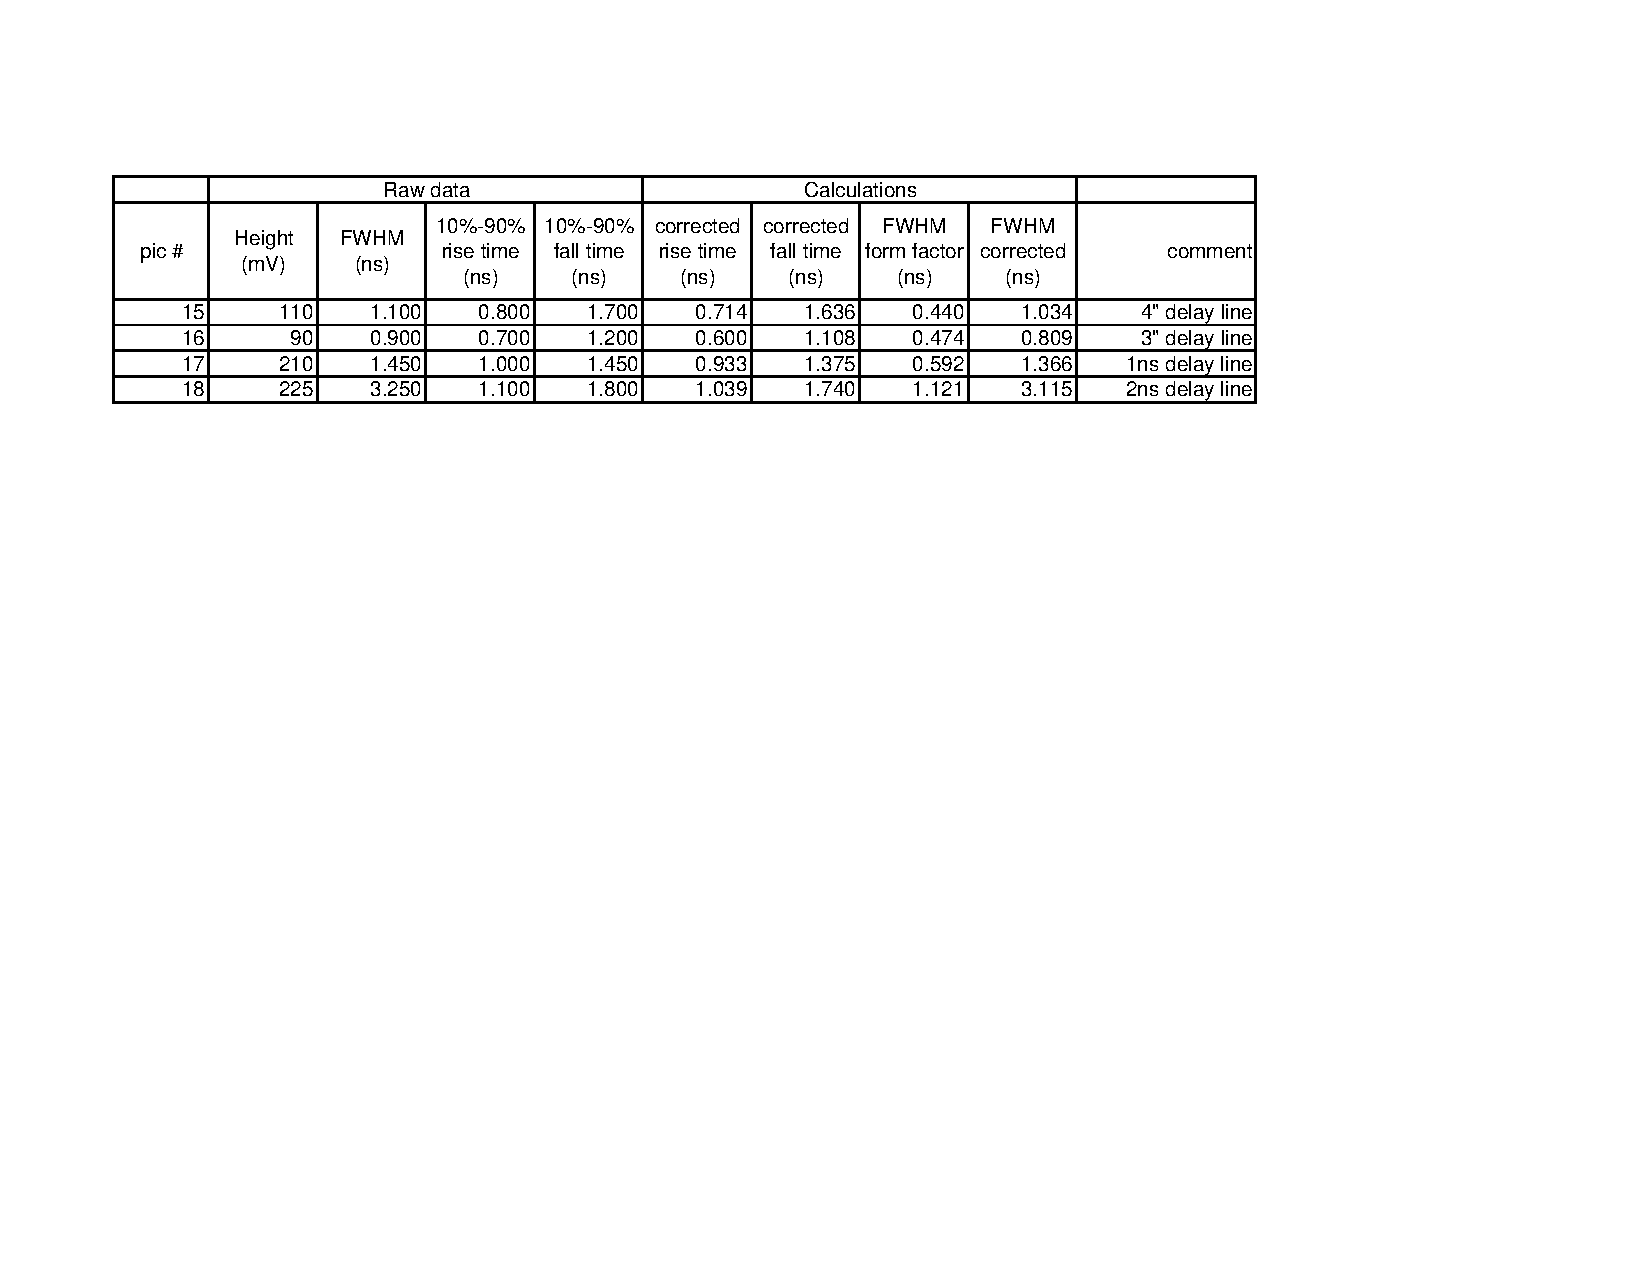
\includegraphics[bb=10 400 605 550]
{delay_lines/delay_lines.pdf}
}
\caption[Pulse length data/calculation table]{Pulse length data/calculation table. Data resulting from various delay lines are corrected for the limited temporal properties of the data acquisition system. The 1ns delay line is 7 7/8'' long and the 2ns delay line is 15 3/4'' long (from connector tip to connector tip).}
\label{delay lines}
\end{figure}
%----------------------------------------------------------------------------

%----------------------------------------------------------------------------
The dye laser generates 535.892nm output (held within 2 picometers by the ``LambdaLok'' feature of the dye laser) at 20Hz with 5ns pulse lengths using a Coumarin 153 dye pumped with a tripled Nd:YAG (355nm) beam. In order to shape the pulsed dye laser output with the Pockels cell, the YAG pump is synchronized with the Hg pulser (which runs the Pockels cell) so that the cell activates at the exact same time the dye laser pulse traverses the crossed polarizers (in the case of the dye laser, we use two polarizing cube beam splitters from Lambda Research Optics) and the cell. This is accomplished through the use of three HP 8015A pulse generators and a few delay lines. Pulser \#1 is designated the ``clock generator'' and triggers the Hg pulser and the flashlamps in the YAG.

%----------------------------------------------------------------------------
%----------------------------------------------------------------------------
%bb defines the bounding box for the pdf
%viewport defines the area of the pdf used
%in sidewaysfigure the last entry in bb moves the caption toward/away the pic
%in sidewaysfigure the second entry in bb moves the pic toward/away the caption
%----------------------------------------------------------------------------
\begin{figure}
\scalebox{0.8}[0.8]{
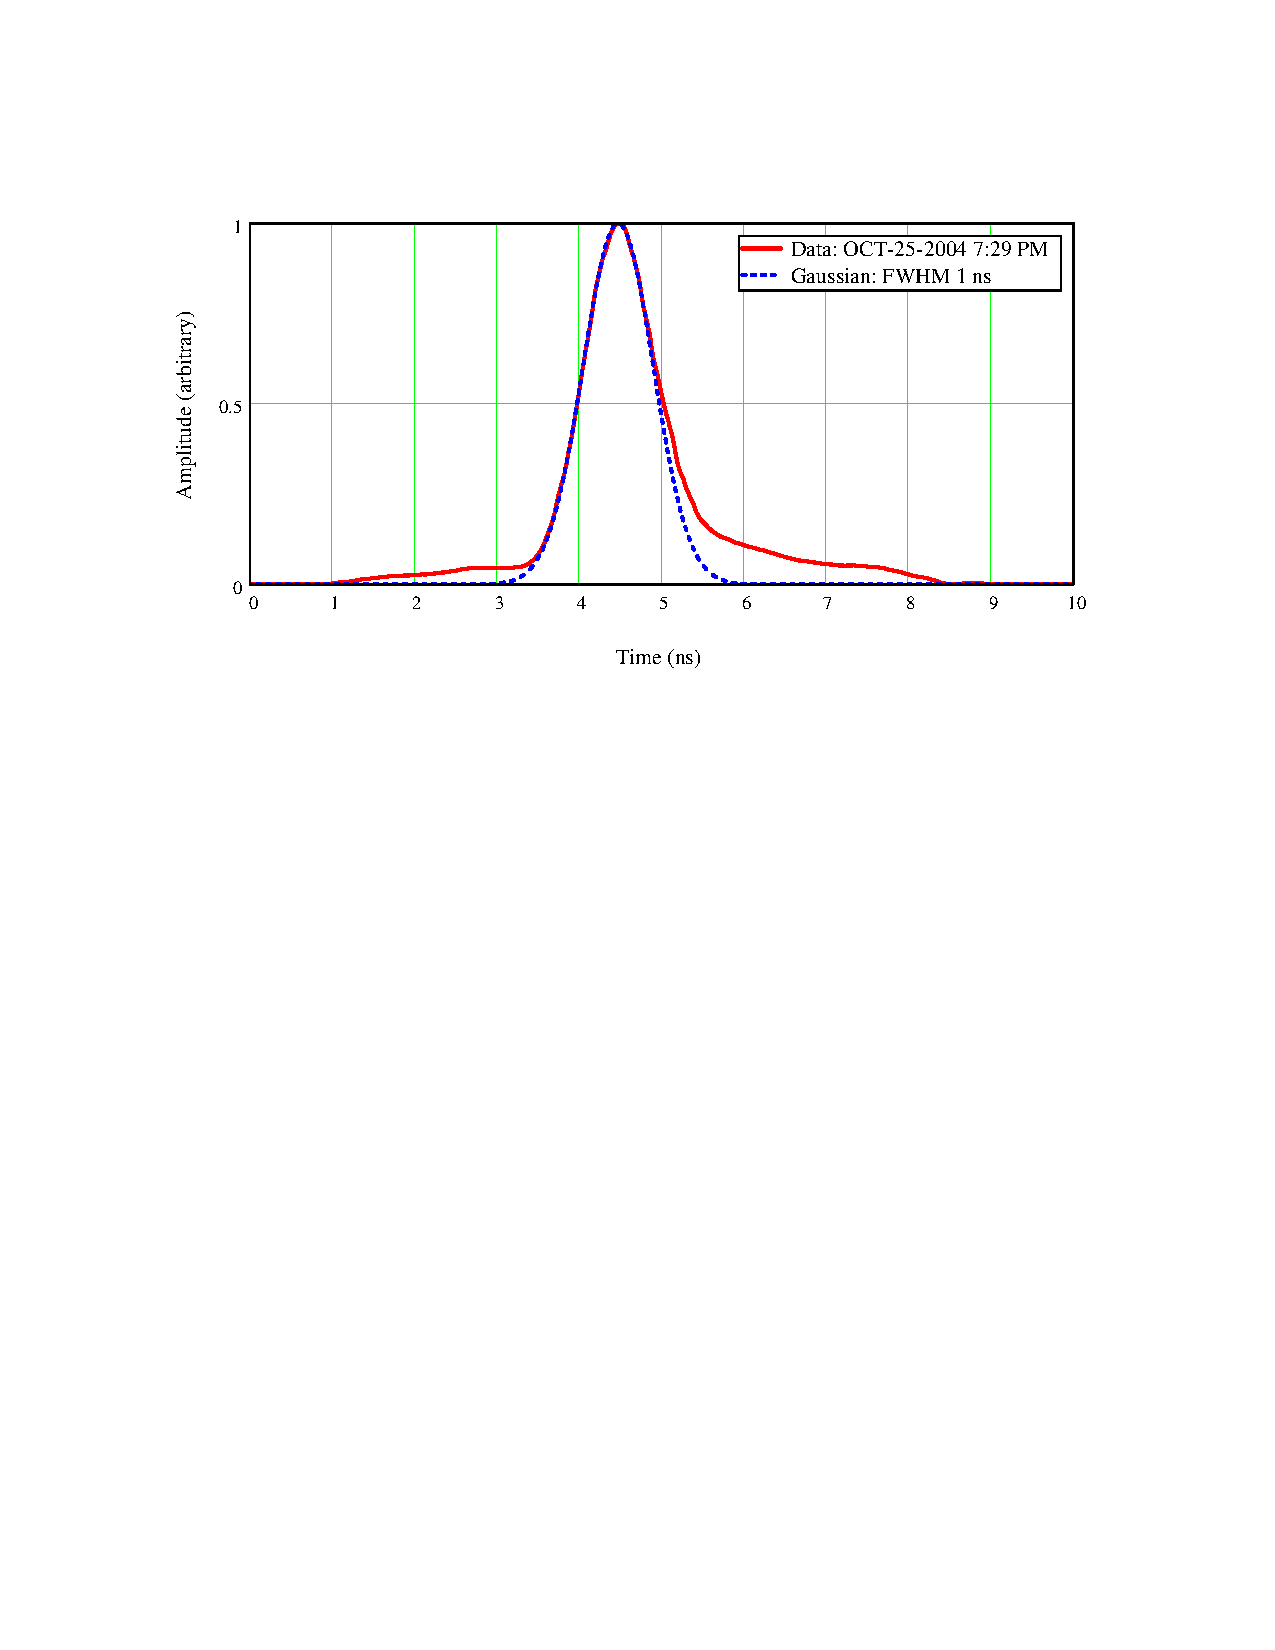
\includegraphics[bb=35 467 523 689]
{temporal_profiles/temporal_profiles.pdf}
}
\caption[Pockels cell minimum pulse length (temporal profiles)]{Pockels cell minimum pulse length (temporal profiles). Here the data corresponding to a 3'' delay cable is overlaid with a computer generated Gaussian pulse. There is significant leaking before and after the pulse; this perhaps due to the relatively low (manufacturer specified) extinction ratio of 1k:1 for the polarizers (compared to 10k:1 for the polarizers used in the HeNe test) and the mismatch between the design wavelength and the laser wavelength.}
\label{temporal profiles}
\end{figure}
%----------------------------------------------------------------------------

%----------------------------------------------------------------------------
The trigger signal for the Hg pulser is sent directly while the TTL trigger signal for the flashlamps is delayed in pulser \#2 (designated the ``flashlamp delay generator'') by about 1060$\mu$s. This flashlamp delay is varied so that the Q-switch opens near the peak of the flashlamp induced population inversion in the Nd:YAG rods; in our case this was about 340$\mu$s before the Q-switch delay generator (see below) TTL pulse. Upon receiving the trigger signal from the clock generator, the Hg pulser closes in about 1.4ms: the high voltage output pulse is to the Pockels cell through 220' of coax cable (introducing a fixed delay of 300ns) while the trigger output is sent to the Q-switch in the YAG.

%----------------------------------------------------------------------------
%----------------------------------------------------------------------------
%bb defines the bounding box for the pdf
%viewport defines the area of the pdf used
%in sidewaysfigure the last entry in bb moves the caption toward/away the pic
%in sidewaysfigure the second entry in bb moves the pic toward/away the caption
%----------------------------------------------------------------------------
\begin{figure}
\scalebox{0.8}[0.8]{
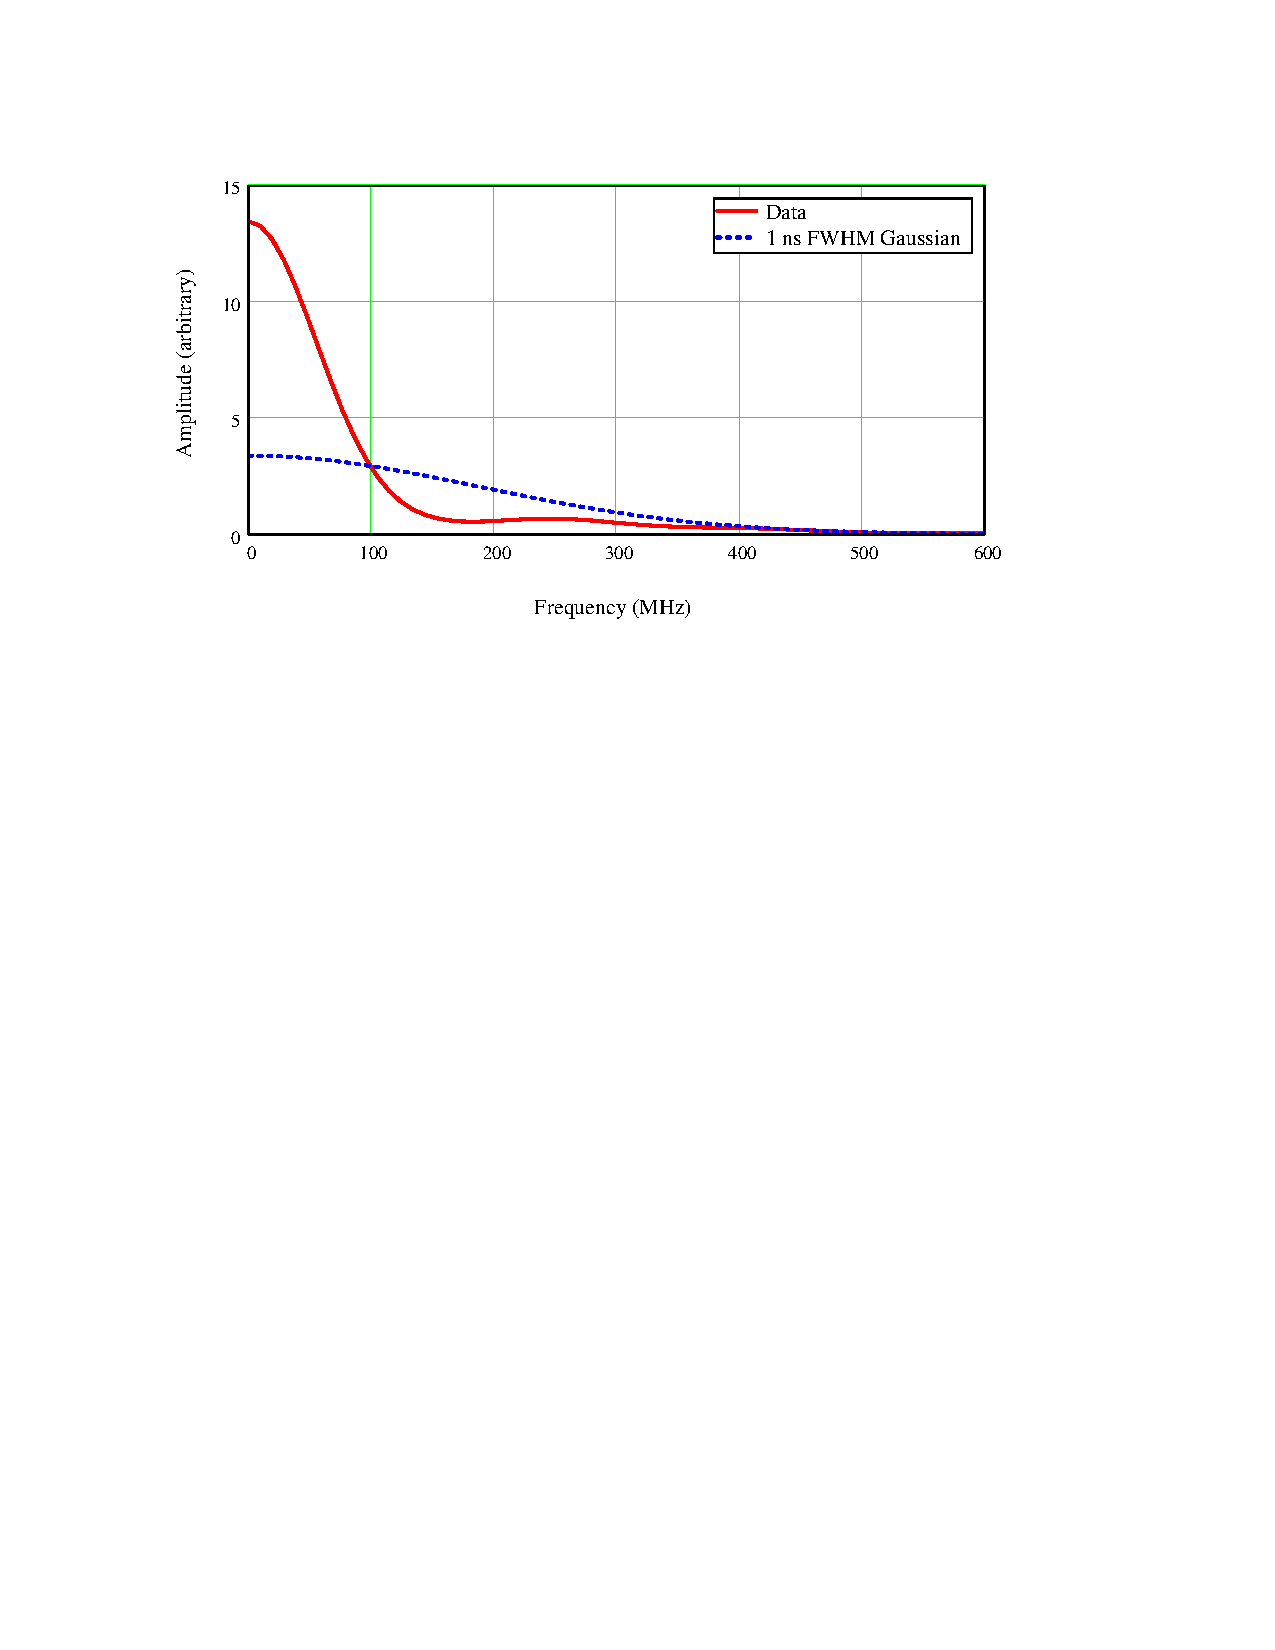
\includegraphics[bb=20 494 481 690]
{spectral_profiles/spectral_profiles.pdf}
}
\caption[Pockels cell minimum pulse length (spectral profiles)]{Pockels cell minimum pulse length (spectral profiles). The power spectrum of the pulses in Figure \ref{temporal profiles} (from a FFT of the temporal profiles) are show here. The leaking results in significant distortion from the optimal Gaussian profile.}
\label{spectral profiles}
\end{figure}
%----------------------------------------------------------------------------

%----------------------------------------------------------------------------
On its way to the YAG's Q-switch input, the trigger signal from the Hg pulser is first sent through a 20dB attenuator and then through pulser \#3 designated the ``Q-switch delay generator'', which adds about 200ns of variable delay. This TTL delay pulse is adjusted to that the subsequent dye laser pulse (the activated Q-switch generates a YAG pulse which in turn generates a dye laser pulse) arrives at the Pockels cell at the exact moment the Pockels cell is activated; in our case this was about 80ns before the Pockels cell is activated. A paper target is placed at the output of the optical switch and the scattered light from the target is observed using a fast photodiode (Electro-optics ET-2000).

For the Hg pulser, a delay line controls the pulse length. The high voltage output pulse is split: half of the signal is sent to the Pockels cell while the other half is sent down an un-terminated (delay line) cable. The high voltage rise reflects inverted from the open end of the cable and returns to cancel the signal sent to the Pockels cell -- this terminates the voltage signal. Thus, the height of the output pulse is half the charging line voltage. Moreover, the pulse length is twice the delay line travel time and the falling edge should have a similar shape as the rising edge. In fact the falling edge shape will always be a distorted version of the rising edge shape due to the inherent frequency dependent attenuation and phase shift introduced by the losses in real cables. We are able to produce fairly symmetric looking pulses out to 200 ns using typical coaxial cable as a delay line.

To determine the minimum pulse length obtainable, a 7'' delay line is successively shortened (using wire cutters) by 1'' increments and the resulting laser pulses at each length are observed on a Tektronix 7104 oscilloscope. The pulse images are recorded using a Polaroid camera attachment for the scope. The Polaroid prints were then analyzed with dividers and a straight edge to determine the height (in mV), the rise and fall times (in ns), and the FWHM (in ns) of each photographed trace. Given the rise/fall time of the photodiode (200/350ps) and the rise/fall time of the oscilloscope (300ps), the rise/fall time and FWHM measurements from the Polaroid images can be corrected using the following formulae
%----------------------------------------------------------------------------
\begin{equation}
t_{r}^2
=
\tau_{r}^2
+
p_{r}^2
+
s_{rf}^2,
\end{equation}
%----------------------------------------------------------------------------
%----------------------------------------------------------------------------
\begin{equation}
t_{f}^2
=
\tau_{f}^2
+
p_{f}^2
+
s_{rf}^2,
\end{equation}
%----------------------------------------------------------------------------
%----------------------------------------------------------------------------
\begin{equation}
t_{w}
=
f_{w}
(t_{r} + t_{f}),
\end{equation}
%----------------------------------------------------------------------------
and
%----------------------------------------------------------------------------
\begin{equation}
\tau_{w}
=
f_{w}
(\tau_{r} + \tau_{f})
\end{equation}
%----------------------------------------------------------------------------
where $p_{r}$ is the photodiode rise time, $p_{f}$ is the photodiode fall time, $p_{r}$ is the photodiode rise time, $s_{rf}$ is the Tektronix 7104 rise/fall time, $t_{r}$ is the measured rise time, $t_{f}$ is the measured fall time, $t_{w}$ is the measured FWHM, $\tau_{r}$ is the corrected rise time, $\tau_{f}$ is the corrected fall time, $f_{w}$ is the FWHM form factor, and $\tau_{w}$ is the corrected FWHM.

We found that a 3'' delay cable produced the best results; see Figure \ref{delay lines} for a data/calculation table. To determine the degree to which the output pulse approximates a Gaussian, a power spectrum of the (uncorrected) temporal envelope is calculated. See Figure \ref{temporal profiles} and \ref{spectral profiles} for the results. It is found that ``leaking'' caused by poor polarizer extinction ratios can significantly distort the power spectrum profile from the Gaussian case.
%----------------------------------------------------------------------------
%----------------------------------------------------------------------------

%----------------------------------------------------------------------------
\subsection{Pinholes}
%----------------------------------------------------------------------------
%----------------------------------------------------------------------------
The envelope for the TEM00 mode from dye laser \#21 is calculated for the beam line described in figures \ref{dye_mileposts} and \ref{conditioning_table}. Equations \ref{free space} and \ref{thin lens} are used to propagate the complex source point $q$ down the beam line. We obtain the following complex source points for key points along the beam line ($\lambda=725$ nm):
%----------------------------------------------------------------------------
\begin{eqnarray}
q_{0}   &=& 1.346  + 8.495i,\\
q_{50}  &=& -1.022 + 0.114i,\\
q_{54}  &=& -3.144 + 5.885i,\\
q_{295} &=& -0.515 + 0.036i,
\end{eqnarray}
%----------------------------------------------------------------------------
where the subscript denotes the milepost at which the complex source is reported. See figure \ref{dye21_to_pinhole} for a plot of the beam envelope up to the pinhole.
%----------------------------------------------------------------------------
% dye21_to_pinhole.tex
% by Troy Hix, May 2005
%----------------------------------------------------------------------------
\begin{figure}
\centering
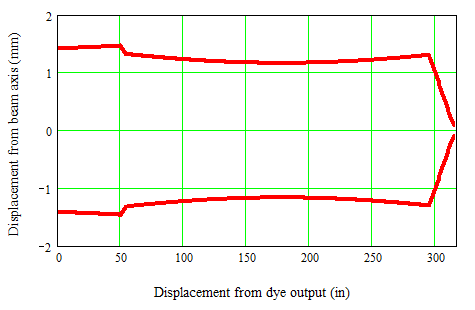
\includegraphics[width=4.00in]
{dye21_to_pinhole/dye21_to_pinhole.png}
\caption{TEM00 envelope for dye laser \#21}
\label{dye21_to_pinhole}
\end{figure} 
%----------------------------------------------------------------------------

%----------------------------------------------------------------------------
%----------------------------------------------------------------------------
%----------------------------------------------------------------------------
%----------------------------------------------------------------------------
%----------------------------------------------------------------------------
The beam lines for the three dye lasers are very similar. So, without corresponding plots like figure \ref{dye21_to_pinhole}, we report the complex source at key points along the beam lines for dye laser \#22 and \#23. For dye laser \#22 we have ($\lambda=628$ nm)
%----------------------------------------------------------------------------
\begin{eqnarray}
q_{0}   &=& 1.346  + 9.808i,\\
q_{50}  &=& -1.016 + 0.099i,\\
q_{55}  &=& -4.008 + 4.493i,\\
q_{344} &=& -0.515 + 0.040i;
\end{eqnarray}
%----------------------------------------------------------------------------
and for dye laser \#23 we have ($\lambda=872$ nm)
%----------------------------------------------------------------------------
\begin{eqnarray}
q_{0}   &=& 1.346  + 7.063i,\\
q_{50}  &=& -1.031 + 0.135i,\\
q_{52.5}&=& -0.707 + 7.018i,\\
q_{280} &=& -0.516 + 0.025i.
\end{eqnarray}
%----------------------------------------------------------------------------
Note that the initial complex source point is slightly different for each laser. This is because the waist was fixed and the Rayleigh parameter was recalculated given the different wavelength of each laser.
%----------------------------------------------------------------------------
%----------------------------------------------------------------------------
%----------------------------------------------------------------------------
%----------------------------------------------------------------------------

%----------------------------------------------------------------------------
%----------------------------------------------------------------------------
The far field diffraction pattern of a uniformly illuminated pinhole is the well known Airy function. The radial displacement $r_1$ of the first minimum some distance $z$ down the beam line is given by \cite{Saleh:1991a}
%----------------------------------------------------------------------------
\begin{equation}
r_1
=
z
\frac
{1.22\lambda}
{2r},
\end{equation}
%----------------------------------------------------------------------------
where $\lambda$ is the wavelength of the incident beam, and $r$ is the pinhole rdius. The Rayleigh range for a circular aperture is \cite{Saleh:1991a}
%----------------------------------------------------------------------------
\begin{equation}
z_R
=
\frac
{\pi r^2}
{\lambda}.
\end{equation}
%----------------------------------------------------------------------------
For distances $z>z_R$ we will assume to be in the far field limit. For the beam line in figure \ref{conditioning_table}, the pinholes (b), (e), and (h) are 0.2 m upstream from +0.2 m lenses. Suppose the pinholes have a diameter of 25 $\mu$m and consider the beam from dye laser \#21 (725 nm). The Rayleigh range for this pinhole is 677 $\mu$m; thus, the lenses are in the far field. At the lens the radial displacement of the first minimum is 7.076 mm, yielding a semi-Gaussian (by placing a 14.2 mm aperture before the +0.2 m lens) beam with a full width of about 14 mm. See figure \ref{spot_size}.
%----------------------------------------------------------------------------
% spot_size.tex
% by Troy Hix, May 2005
%----------------------------------------------------------------------------
\begin{figure}
\centering
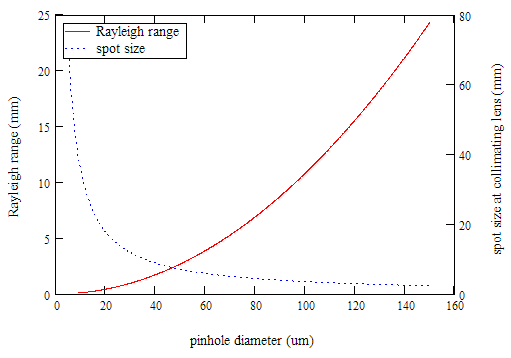
\includegraphics[width=4.00in]
{spot_size/spot_size.png}
\caption[Rayleigh range (724 nm) and spot size vs. pinhole diameter]{Rayleigh range (724 nm) and spot size vs. pinhole diameter. Even with a pinhole as large as 150 $\mu$m the Rayleigh range for the pinhole function is only 24.374 mm while the spot size 20 cm from the pinhole is 2.359 mm in diameter. For a pinhole with a diameter of 50 $\mu$m the Rayleigh range is 2.708 mm and the spot size at 20 cm is 7.076 mm.}
\label{spot_size}
\end{figure} 
%----------------------------------------------------------------------------

%----------------------------------------------------------------------------
%----------------------------------------------------------------------------
%----------------------------------------------------------------------------
\subsubsection{Damage threshold}
%----------------------------------------------------------------------------
In the following analysis we will assume the beams involved have a circular top-hat intensity distributions for simplicity.

Pinholes made to handle high power from standard suppliers typically have a damage threshold of around 1MW/mm$^2$. Given a waist at the pinhole of about 80 $\mu$m, we can only use 4.4 ns pulses with about 100 $\mu$J of energy. The ratio of the area of the pinhole to the total area of the beam implies that only 10\% of the energy incident on the pinhole makes it through. Since the central maximum of the Airy function contains about 84\% of the energy in the pinhole, the beam after the +0.2 m lens can have about 8 $\mu$J of energy at most. This 8 $\mu$J is then run through an aperture before the iodine cell. If this aperture has a radius of around 1 mm then the energy of the beam at the iodine sample is about 160 nJ. This is 2 to 3 orders of magnitude less than our estimate of the energy needed at the iodine sample for coherent control. Thus, an ordinary metallic pinhole may not be the best choice. A glass fiber will be better: the only limit is the surface damage threshold of the glass: around 5GW/cm$^2$. See figure \ref{energy}.
%----------------------------------------------------------------------------
% energy.tex
% by Troy Hix, May 2005
%----------------------------------------------------------------------------
\begin{figure}
\centering
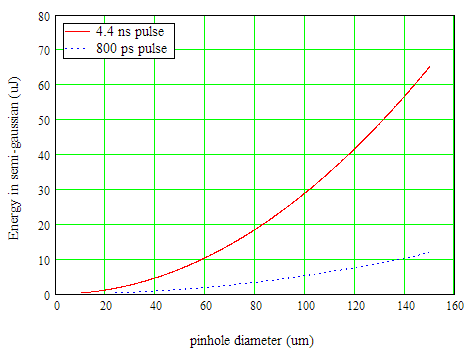
\includegraphics[width=4.00in]
{energy/energy.png}
\caption{Energy in the Airy function central max vs. pinhole size.}
\label{energy}
\end{figure} 
%----------------------------------------------------------------------------

%----------------------------------------------------------------------------
%----------------------------------------------------------------------------
%----------------------------------------------------------------------------

%----------------------------------------------------------------------------
\subsection{General discussion on etalon efficiency}
%----------------------------------------------------------------------------
%----------------------------------------------------------------------------
We seek a relationship between the resolution and power transmittance of a etalon type interferometer. Interferometers are subject to the localization property from (spatial) Fourier analysis:
%----------------------------------------------------------------------------
\begin{equation}
\Delta x
\propto
\frac{1}{\Delta k}
\end{equation}
%----------------------------------------------------------------------------
where $\Delta x$ is the width of some localized feature in space and $\Delta k$ is the corresponding width in inverse space. In optical interferometers, $\Delta k$ is the ``resolution'' of the resulting interferogram and $\Delta x$ is the largest optical path length difference associated with the interferometer. In the case of a etalon type interferometer $\Delta x$ is equal to the optical path length of the etalon medium times the number of passes the reflection coatings can support; thus, we will assume
%----------------------------------------------------------------------------
\begin{equation}
\Delta x
\propto
n
\equiv
\frac{1}{1-R}
\end{equation}
%----------------------------------------------------------------------------
where $n$ is the number of passes and $R$ is the reflectance transmission of the etalon coating. This is reasonable when one considers that this implies $\Delta x$ diverges toward infinity as $R$ approaches unity and the fact that if $R=0.9$ then one would expect about ten reflections until the beam would no longer contribute significantly to the etalon's interference effect.

The power transmittance of the etalon is a function of the losses at each mirror and the bulk absorption in the etalon material. Clearly, a reasonable form for the power transmission is
%----------------------------------------------------------------------------
\begin{equation}
T
\propto
\gamma^{n}
=
\gamma^{1/(1-R)}
=
\gamma^{\zeta \Delta x}.
\end{equation}
%----------------------------------------------------------------------------
where $\gamma$ is the transmission of one pass (representing the effects of reflection and bulk losses) and $\zeta$ is a constant with units of inverse length. Moreover, application of the localization property gives
%----------------------------------------------------------------------------
\begin{equation}
T
\propto
\gamma^{\zeta/\Delta k}.
\end{equation}
%----------------------------------------------------------------------------
Thus, we see that because $\gamma<1$, any attempt to increase the resolution of the instrument will result in a reduction in power transmission.
%----------------------------------------------------------------------------
%----------------------------------------------------------------------------

%----------------------------------------------------------------------------
\subsection{Confocal etalon test}
%----------------------------------------------------------------------------
%----------------------------------------------------------------------------
%----------------------------------------------------------------------------
%----------------------------------------------------------------------------
%bb defines the bounding box for the pdf
%viewport defines the area of the pdf used
%in sidewaysfigure the last entry in bb moves the caption toward/away the pic
%in sidewaysfigure the second entry in bb moves the pic toward/away the caption
%----------------------------------------------------------------------------
\begin{figure}
\scalebox{0.8}[0.8]{
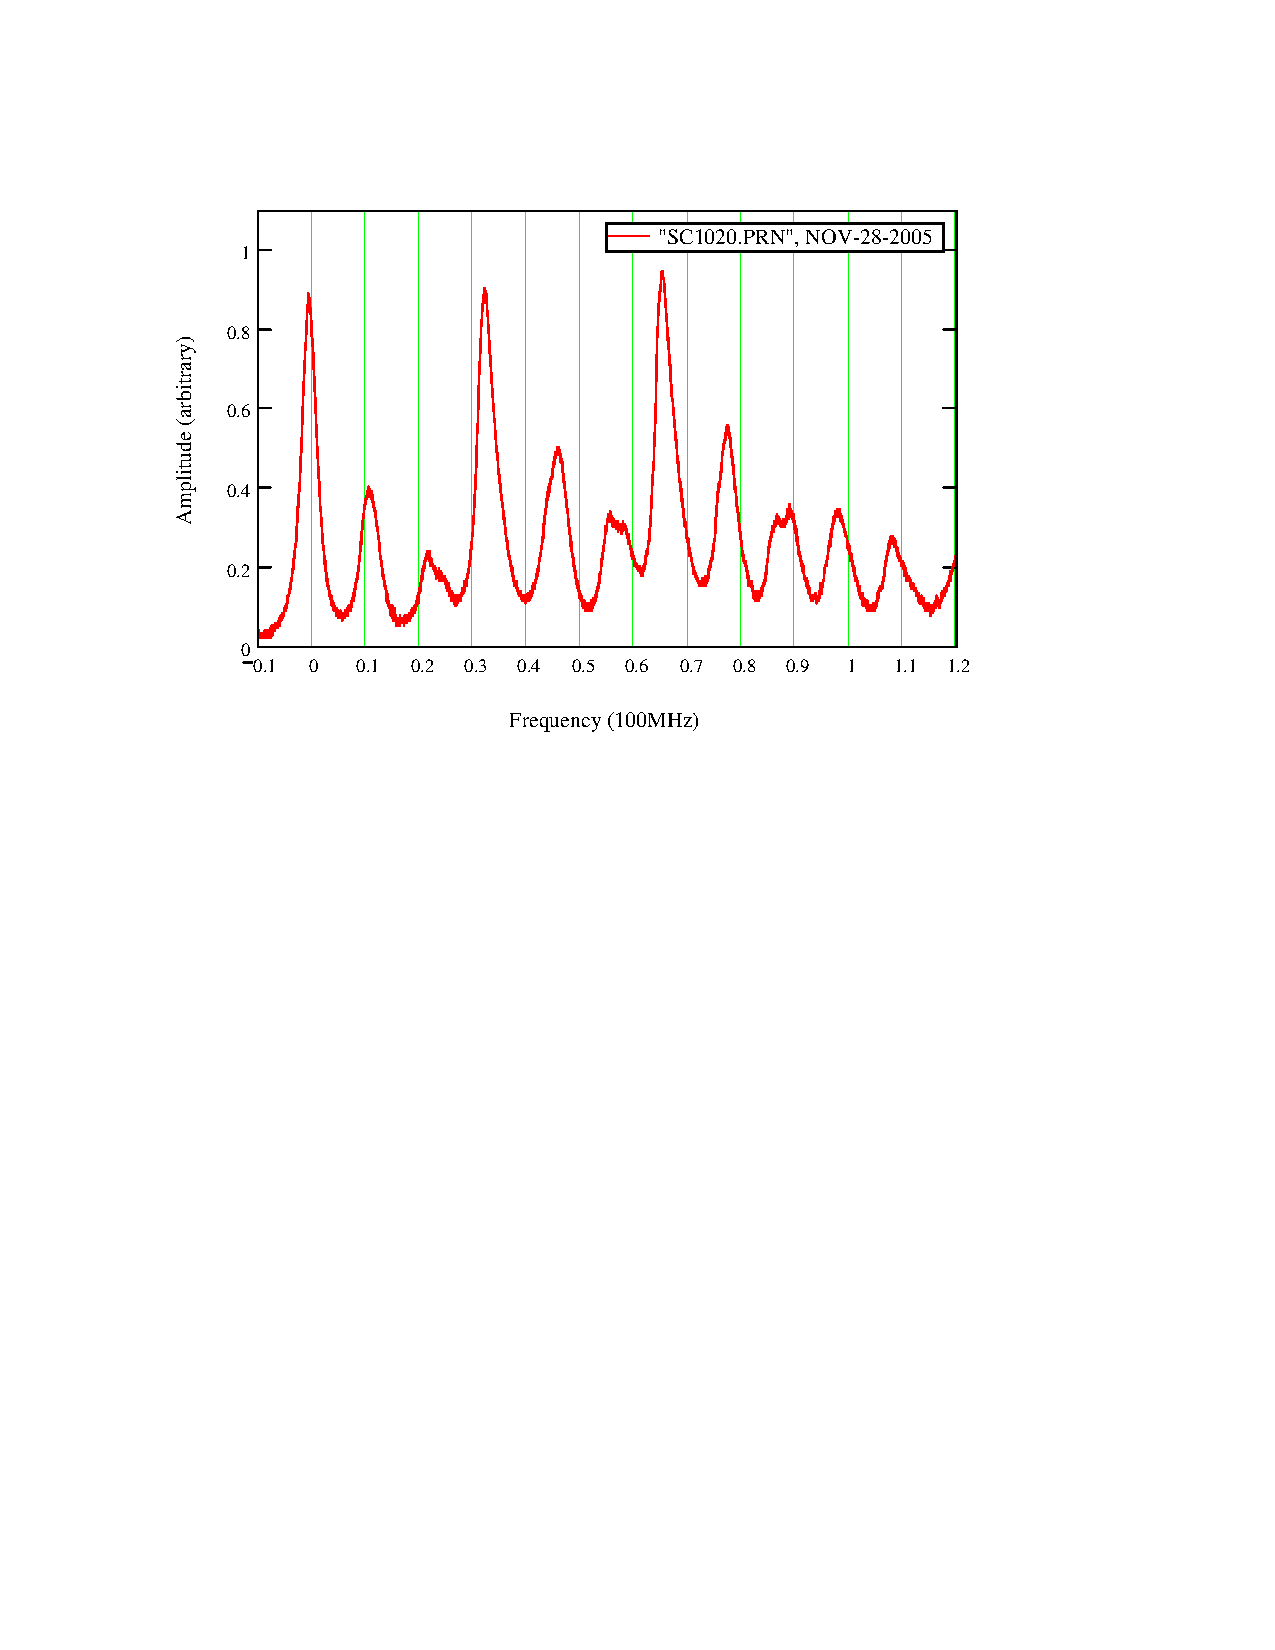
\includegraphics[bb=15 440 489 752]
{near_confocal/near_confocal.pdf}
}
\caption[Green HeNe transmission through a scaned near confocal etalon]{Green HeNe transmission through a scaned near confocal etalon}
\label{near_confocal}
\end{figure}
%----------------------------------------------------------------------------

%----------------------------------------------------------------------------
%----------------------------------------------------------------------------
%bb defines the bounding box for the pdf
%viewport defines the area of the pdf used
%in sidewaysfigure the last entry in bb moves the caption toward/away the pic
%in sidewaysfigure the second entry in bb moves the pic toward/away the caption
%----------------------------------------------------------------------------
\begin{figure}
\scalebox{0.8}[0.8]{
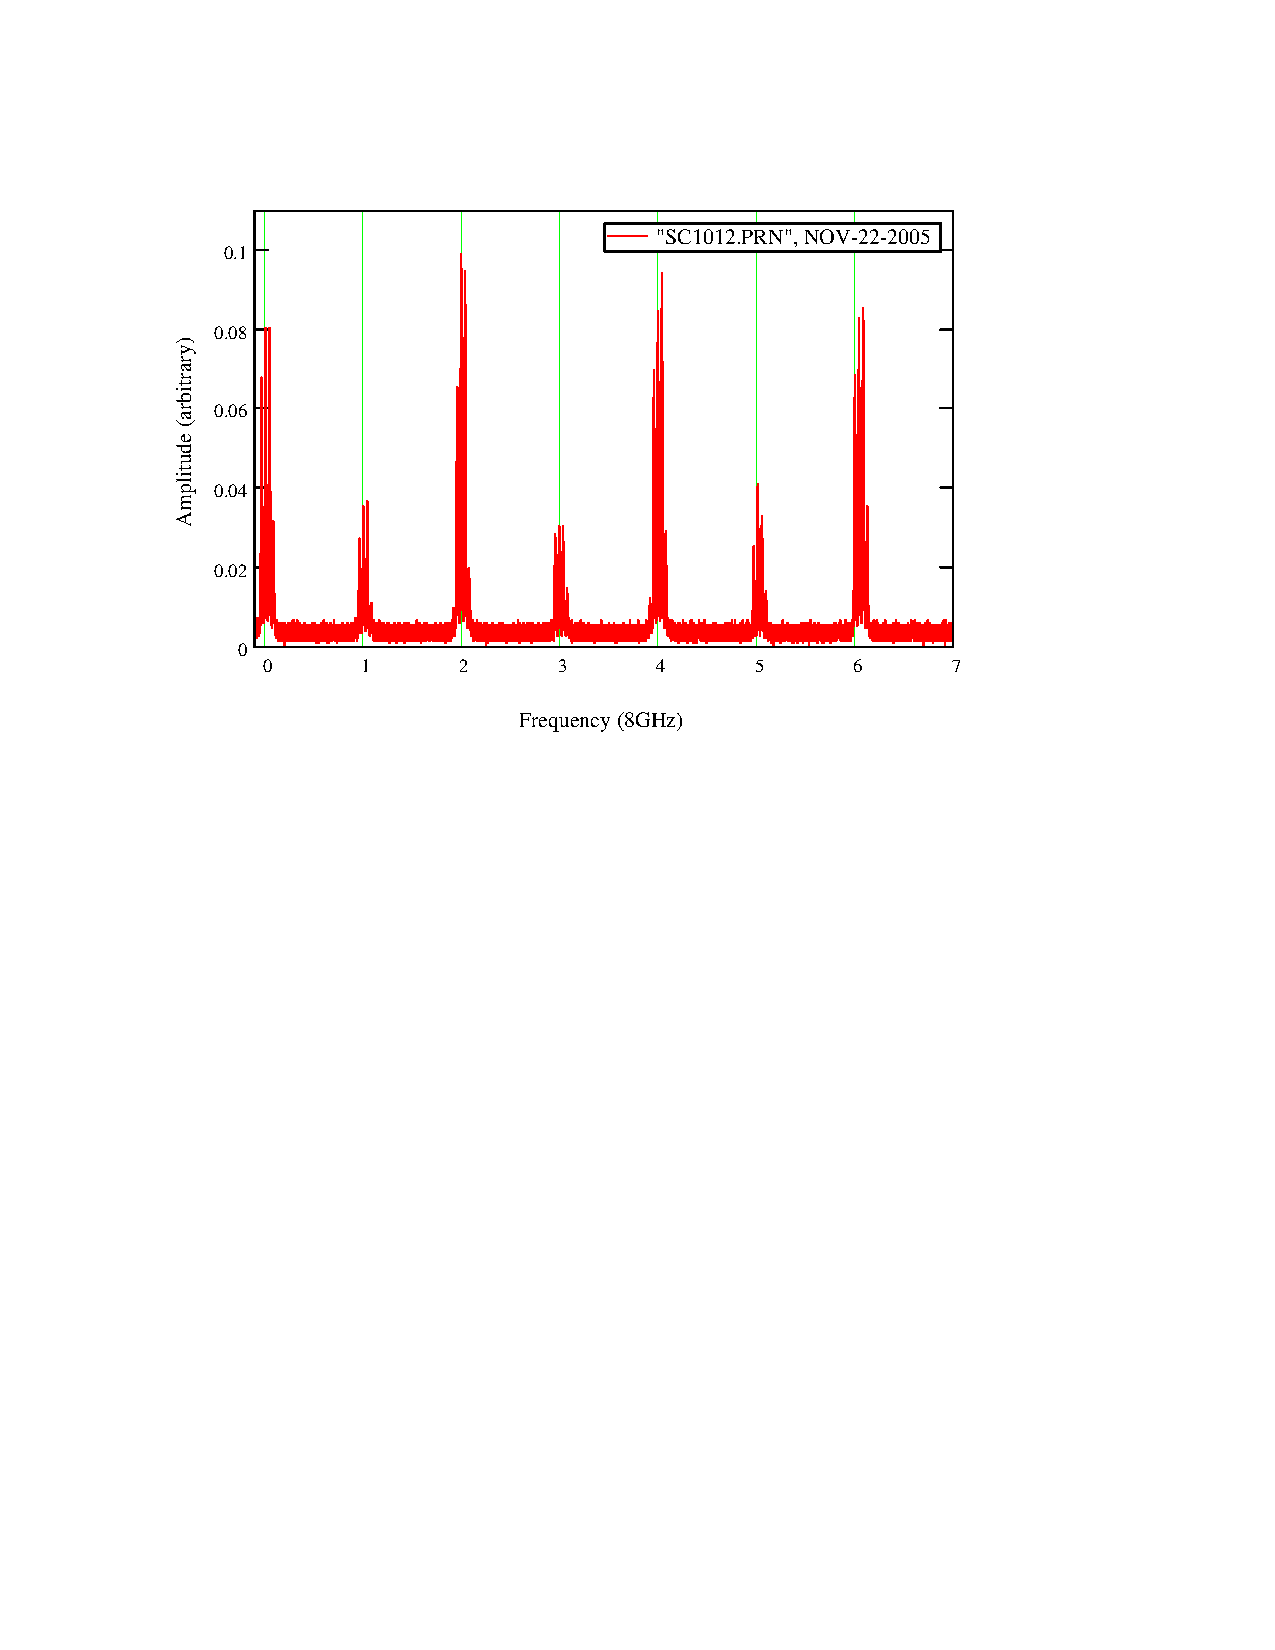
\includegraphics[bb=15 440 489 752]
{confocal_all/confocal_all.pdf}
}
\caption[Green HeNe transmission through a scanned confocal etalon]{Green HeNe transmission through a scanned confocal etalon}
\label{confocal_all}
\end{figure}
%----------------------------------------------------------------------------

%----------------------------------------------------------------------------
%----------------------------------------------------------------------------
%bb defines the bounding box for the pdf
%viewport defines the area of the pdf used
%in sidewaysfigure the last entry in bb moves the caption toward/away the pic
%in sidewaysfigure the second entry in bb moves the pic toward/away the caption
%----------------------------------------------------------------------------
\begin{figure}
\scalebox{0.8}[0.8]{
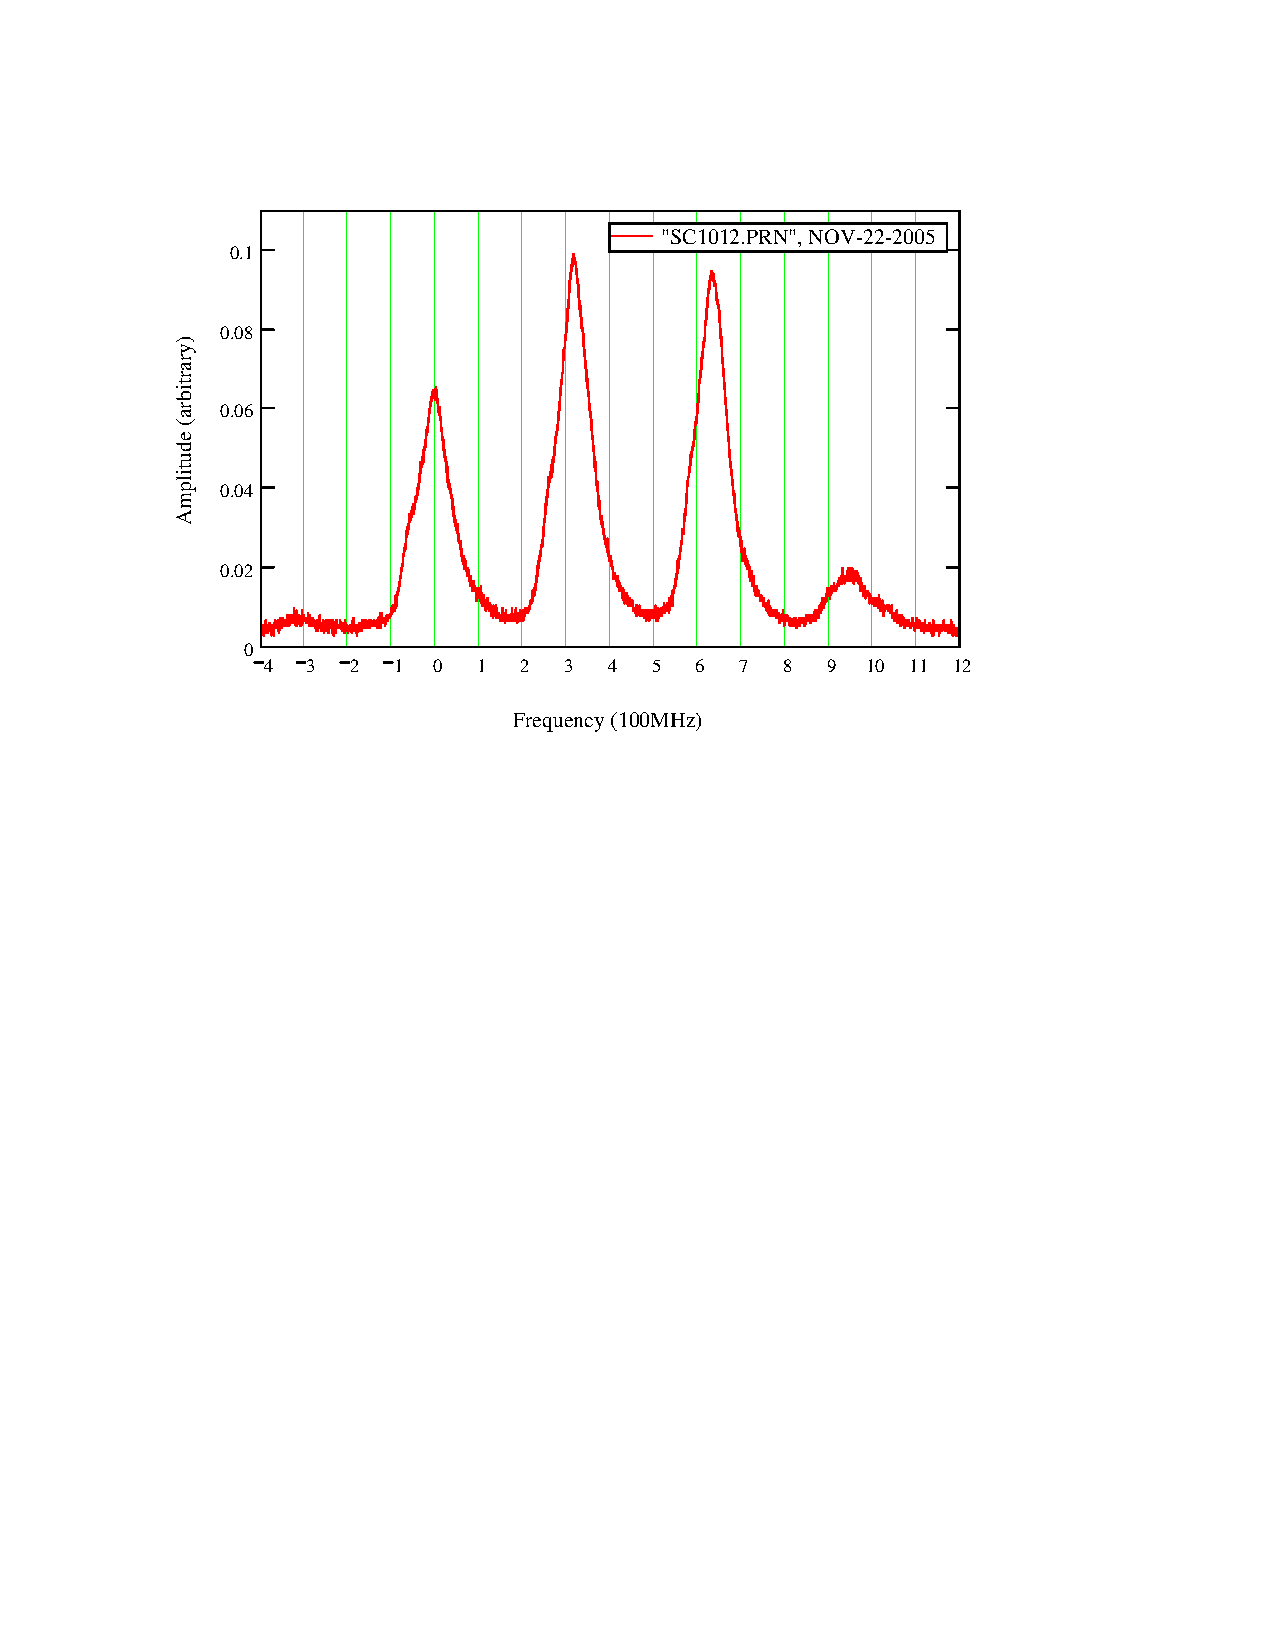
\includegraphics[bb=15 440 489 752]
{confocal_zoom/confocal_zoom.pdf}
}
\caption[Green HeNe transmission through a scanned confocal etalon (zoom)]{Green HeNe transmission through a scanned confocal etalon (zoom). The green HeNe mode spacing is 326 MHz and the etalon mode width is 100 MHz.}
\label{confocal_zoom}
\end{figure}
%----------------------------------------------------------------------------

%----------------------------------------------------------------------------
%----------------------------------------------------------------------------

%----------------------------------------------------------------------------
%----------------------------------------------------------------------------
%----------------------------------------------------------------------------
%----------------------------------------------------------------------------
%----------------------------------------------------------------------------
